\documentclass[11pt]{beamer} % add [handout] to ignore \pause,\only, and \visible
\usetheme{default} % literally the same as EastLansing but with green text instead of blue
\usecolortheme{spruce} % "Spartan" green
\setbeamertemplate{page number in head/foot}{} % no slide numbers
\setbeamertemplate{bibliography item}[text]
\setbeamertemplate{caption}{\raggedright\insertcaption\par}
\setbeamertemplate{navigation symbols}{}
\definecolor{darkgreenlansing}{rgb}{0, 0.31764705882, 0.15686274509}
\definecolor{lightgreenlansing}{rgb}{0.851, 0.91, 0.882}
\definecolor{codegrey}{rgb}{0.8,0.8,0.8}
\setbeamercolor{button}{bg=darkgreenlansing,fg=white}
\setbeamertemplate{items}{\color{darkgreenlansing}$\blacktriangleright$}
\usefonttheme[onlymath]{serif}

\usepackage{hyperref} % for linking
\usepackage{lmodern} % for better font rendering
\usepackage{lipsum} % for generating dummy text
\usepackage{xcolor} % for colored text
\usepackage{framed}
\usepackage{mathabx} % for squiggle arrow
\usepackage{siunitx} % for SI units
\colorlet{shadecolor}{lightgreenlansing!50}

\newcommand{\highlight}[1]{%
  \colorbox{lightgreenlansing!50}{$\displaystyle#1$}}

\usepackage{cancel} % for strikethrough
\usepackage{svg} % for svg images
\usepackage{listings} % for code blocks
\usepackage{xparse} % for custom commands
\usepackage{graphicx} % for images
\usepackage{adjustbox} % for adjusting images
\usepackage[normalem]{ulem} % for \sout{} and to remove underlining from hyperlinks
\usepackage{pict2e}

\makeatletter
\newcommand{\crossout}[1]{%
  \begingroup
  \settowidth{\dimen@}{#1}%
  \setlength{\unitlength}{0.05\dimen@}%
  \settoheight{\dimen@}{#1}%
  \count@=\dimen@
  \divide\count@ by \unitlength
  \begin{picture}(0,0)
  \put(0,0){\line(20,\count@){20}}
  \put(0,\count@){\line(20,-\count@){20}}
  \end{picture}%
  #1%
  \endgroup
}
\makeatother
\usepackage[linewidth=1pt]{mdframed} % for frames
\usepackage[backend=biber,style=authoryear,maxnames=2]{biblatex} % for citations
\addbibresource{\jobname.bib} % with extension
\AtEveryBibitem{%
   \clearfield{month}
   \clearfield{series}
   \clearfield{venue}
   \clearname{editor}
   %\clearlist{publisher}
   \clearlist{location} % alias to field 'address'
   %\clearfield{doi}
   \clearfield{url}
   \clearfield{venue}
   \clearfield{issn}
   \clearfield{isbn}
   \clearfield{urldate}
   \clearfield{eventdate}
   \clearfield{title}
   %\clearfield{pages}
   %\clearfield{booktitle}
   %\clearfield{journaltitle}
   %\clearfield{number}
   %\clearfield{volume}
}
\AtBeginBibliography{\tiny}

% add journal to citations
\renewbibmacro*{cite}{%
  \iffieldundef{shorthand}
    {\ifthenelse{\ifnameundef{labelname}\OR\iffieldundef{labelyear}}
       {\usebibmacro{cite:label}%
        \setunit{\printdelim{nonameyeardelim}}}
       {\printnames{labelname}%
        \setunit{\printdelim{nameyeardelim}}}%
     \usebibmacro{cite:labeldate+extradate}%
     \setunit{\addcomma\space}%
     \usebibmacro{journal}}
    {\usebibmacro{cite:shorthand}}}

\NewDocumentCommand{\expectation}{m o}{%
\IfValueTF{#2}{%
    \ensuremath{\left\langle #1 \middle| #2 \middle| #1\right\rangle}%
}
{%
    \ensuremath{\left\langle #1 \right\rangle}%
}
}

\def\IsInteger#1{%
  TT\fi
  \begingroup \lccode`\-=`\0 \lccode`+=`\0
    \lccode`\1=`\0 \lccode`\2=`\0 \lccode`\3=`\0
    \lccode`\4=`\0 \lccode`\5=`\0 \lccode`\6=`\0
    \lccode`\7=`\0 \lccode`\8=`\0 \lccode`\9=`\0
  \lowercase{\endgroup
    \expandafter\ifx\expandafter\delimiter
    \romannumeral0\string#1}\delimiter
}
\newcommand{\ord}[1]{%
    \if\IsInteger{#1}%
        \ifthenelse{1=#1}
        {%
            $1^{\mathrm{st}}$%
        }%
        {%
            \ifthenelse{2=#1}
            {%
                $2^{\mathrm{nd}}$%
            }%
            {%
                \ifthenelse{3=#1}
                {%
                    $3^{\mathrm{rd}}$%
                }%
                {%
                    $#1^{\mathrm{th}}$%
                }%
            }%
        }%
    \else%
        {%
            $#1^{\mathrm{th}}$%
        }%
    \fi%
}

\DeclareMathOperator*{\argmax}{arg\,max}
\DeclareMathOperator*{\argmin}{arg\,min}


\newcommand\hcancel[2][black]{\setbox0=\hbox{$#2$}%
\rlap{\raisebox{.45\ht0}{\textcolor{#1}{\rule{\wd0}{1pt}}}}#2}
\newcommand{\bra}[1]{\ensuremath{\left\langle#1\right|}}
\newcommand{\ket}[1]{\ensuremath{\left|#1\right\rangle}}
\newcommand{\mbf}[1]{\ensuremath{\mathbf{#1}}}
\newcommand{\Sx}{\ensuremath{\left\langle S_x\right\rangle}}
\newcommand{\Sy}{\ensuremath{\left\langle S_y\right\rangle}}
\newcommand{\Sxsq}{\ensuremath{\left\langle S_x^2\right\rangle}}
\newcommand{\Sxsqt}{\ensuremath{\left\langle S_x^2(t)\right\rangle}}
\newcommand{\Sysq}{\ensuremath{\left\langle S_y^2\right\rangle}}
\newcommand{\Sysqt}{\ensuremath{\left\langle S_y^2(t)\right\rangle}}
\newcommand{\gx}{\ensuremath{\gamma_x}}
\newcommand{\gy}{\ensuremath{\gamma_y}}
\newcommand{\Jij}{\ensuremath{J_{ij}}}
\newcommand{\SDsq}{\ensuremath{\left\langle S_D^2\right\rangle}}
\newcommand{\SSsq}{\ensuremath{\left\langle S_S^2\right\rangle}}
\newcommand{\bigO}[1]{\ensuremath{\mathcal{O}\left(#1\right)}}
\newcommand{\nxn}[1]{\ensuremath{#1\times #1}}
\newcommand{\abs}[1]{\ensuremath{\left|#1\right|}}
\newcommand{\norm}[1]{\ensuremath{\left\|#1\right\|}}

\newcommand{\trainable}[1]{\ensuremath{\textcolor{darkgreenlansing}{\underline{#1}}}}

\usepackage{filecontents}
\begin{filecontents}[overwrite]{\jobname.bib}
@misc{feinashley2024single,
      title={A Single Graph Convolution Is All You Need: Efficient Grayscale Image Classification}, 
      author={Jacob Fein-Ashley and Tian Ye and Sachini Wickramasinghe and Bingyi Zhang and Rajgopal Kannan and Viktor Prasanna},
      year={2024},
      eprint={2402.00564},
      archivePrefix={arXiv},
      primaryClass={cs.CV}
}
@misc{cohen2017emnist,
      title={EMNIST: an extension of MNIST to handwritten letters}, 
      author={Gregory Cohen and Saeed Afshar and Jonathan Tapson and André van Schaik},
      year={2017},
      eprint={1702.05373},
      archivePrefix={arXiv},
      primaryClass={cs.CV}
}
@misc{cook2024parametric,
      title={Parametric Matrix Models},
      author={Patrick Cook and Danny Jammooa and Morten Hjorth-Jensen and Daniel D. Lee and Dean Lee},
      year={2024},
      eprint={2401.11694},
      archivePrefix={arXiv},
      primaryClass={cs.LG},
      howpublished = {\url{https://arxiv.org/abs/2401.11694}}
}
@article{DFrame,
  title = {Eigenvector Continuation with Subspace Learning},
  author = {Frame, Dillon and He, Rongzheng and Ipsen, Ilse and Lee, Daniel and Lee, Dean and Rrapaj, Ermal},
  journal = {Phys. Rev. Lett.},
  volume = {121},
  issue = {3},
  pages = {032501},
  numpages = {5},
  year = {2018},
  month = {Jul},
  publisher = {American Physical Society},
  doi = {10.1103/PhysRevLett.121.032501},
  url = {https://link.aps.org/doi/10.1103/PhysRevLett.121.032501}
}

@article{ASarkar,
  title = {Convergence of Eigenvector Continuation},
  author = {Sarkar, Avik and Lee, Dean},
  journal = {Phys. Rev. Lett.},
  volume = {126},
  issue = {3},
  pages = {032501},
  numpages = {6},
  year = {2021},
  month = {Jan},
  publisher = {American Physical Society},
  doi = {10.1103/PhysRevLett.126.032501},
  url = {https://link.aps.org/doi/10.1103/PhysRevLett.126.032501}
}

@article{SKONIG,
title = {Eigenvector continuation as an efficient and accurate emulator for uncertainty quantification},
journal = {Physics Letters B},
volume = {810},
pages = {135814},
year = {2020},
issn = {0370-2693},
doi = {https://doi.org/10.1016/j.physletb.2020.135814},
url = {https://www.sciencedirect.com/science/article/pii/S0370269320306171},
author = {S. König and A. Ekström and K. Hebeler and D. Lee and A. Schwenk},
}
@article{vanderMaaten08,
author = {van der Maaten, Laurens and Hinton, Geoffrey},
year = {2008},
month = {11},
pages = {2579-2605},
title = {Viualizing data using t-{SNE}},
volume = {9},
journal = {Journal of Machine Learning Research}
}

@article{vanderMaaten14,
  author  = {Laurens van der Maaten},
  title   = {Accelerating t-{SNE} using Tree-Based Algorithms},
  journal = {Journal of Machine Learning Research},
  year    = {2014},
  volume  = {15},
  number  = {93},
  pages   = {3221--3245},
  url     = {http://jmlr.org/papers/v15/vandermaaten14a.html}
}

@article{vanderMaaten09,
author = {van der Maaten, Laurens},
year = {2009},
month = {01},
pages = {384-391},
title = {Learning a Parametric Embedding by Preserving Local Structure.},
volume = {5},
journal = {Journal of Machine Learning Research - Proceedings Track}
}

@misc{ji2019invariant,
      title={Invariant Information Clustering for Unsupervised Image Classification and Segmentation},
      author={Xu Ji and João F. Henriques and Andrea Vedaldi},
      year={2019},
      eprint={1807.06653},
      archivePrefix={arXiv},
      primaryClass={cs.CV}
}

@misc{paperswithcode,
  title = {Papers with Code},
  howpublished = {\url{https://paperswithcode.com/}},
  note = {Accessed: 02-09-2024}
}

@misc{MSFTnuclear,
  title = {{M}icrosoft is going nuclear to power its {AI} ambitions},
  howpublished = {\url{https://www.theverge.com/2023/9/26/23889956/microsoft-next-generation-nuclear-energy-smr-job-hiring}},
  note = {Accessed: 02-09-2024}
}

@misc{OurWorldInData,
    title = {Parameters in notable artificial intelligence systems},
    howpublished = {\url{https://ourworldindata.org/grapher/artificial-intelligence-parameter-count}},
    note = {Accessed: 05-08-2024}
}

@misc{CIFAR,
  title={Learning Multiple Layers of Features from Tiny Images},
  author={Alex Krizhevsky},
  year={2009},
  url={https://api.semanticscholar.org/CorpusID:18268744},
  howpublished={\url{https://api.semanticscholar.org/CorpusID:18268744}}
}

@ARTICLE{MNIST,
  author={Lecun, Y. and Bottou, L. and Bengio, Y. and Haffner, P.},
  journal={Proceedings of the IEEE}, 
  title={Gradient-based learning applied to document recognition}, 
  year={1998},
  volume={86},
  number={11},
  pages={2278-2324},
  keywords={Neural networks;Pattern recognition;Machine learning;Optical character recognition software;Character recognition;Feature extraction;Multi-layer neural network;Optical computing;Hidden Markov models;Principal component analysis},
  doi={10.1109/5.726791}}

@ARTICLE{FashionMNIST,
       author = {{Xiao}, Han and {Rasul}, Kashif and {Vollgraf}, Roland},
        title = "{Fashion-MNIST: a Novel Image Dataset for Benchmarking Machine Learning Algorithms}",
      journal = {arXiv e-prints},
     keywords = {Computer Science - Machine Learning, Computer Science - Computer Vision and Pattern Recognition, Statistics - Machine Learning},
         year = 2017,
        month = aug,
          eid = {arXiv:1708.07747},
        pages = {arXiv:1708.07747},
          doi = {10.48550/arXiv.1708.07747},
archivePrefix = {arXiv},
       eprint = {1708.07747},
 primaryClass = {cs.LG},
       adsurl = {https://ui.adsabs.harvard.edu/abs/2017arXiv170807747X},
      adsnote = {Provided by the SAO/NASA Astrophysics Data System}
}
@article{DNNResNet,
  title = {Trainable Activations for Image Classification},
  author = {Pishchik, Evgenii},
  orcid = {https://orcid.org/0000-0001-6614-4419},
  url = {https://github.com/Pe4enIks/TrainableActivation},
  year = {2023},
  doi = {10.20944/preprints202301.0463.v1},
}
@article{kMobileNet, title={Grouped Pointwise Convolutions Reduce Parameters in Convolutional Neural Networks}, volume={28}, url={https://mendel-journal.org/index.php/mendel/article/view/169}, DOI={10.13164/mendel.2022.1.023}, number={1}, journal={MENDEL}, author={Schwarz Schuler, Joao Paulo and Romani, Santiago and Abdel-Nasser, Mohamed and Rashwan, Hatem and Puig, Domenec}, year={2022}, month={Jun.}, pages={23-31} }
@article{HYVARINEN2000411,
title = {Independent component analysis: algorithms and applications},
journal = {Neural Networks},
volume = {13},
number = {4},
pages = {411-430},
year = {2000},
issn = {0893-6080},
doi = {https://doi.org/10.1016/S0893-6080(00)00026-5},
url = {https://www.sciencedirect.com/science/article/pii/S0893608000000265},
author = {A. Hyvärinen and E. Oja},
keywords = {Independent component analysis, Projection pursuit, Blind signal separation, Source separation, Factor analysis, Representation},
abstract = {A fundamental problem in neural network research, as well as in many other disciplines, is finding a suitable representation of multivariate data, i.e. random vectors. For reasons of computational and conceptual simplicity, the representation is often sought as a linear transformation of the original data. In other words, each component of the representation is a linear combination of the original variables. Well-known linear transformation methods include principal component analysis, factor analysis, and projection pursuit. Independent component analysis (ICA) is a recently developed method in which the goal is to find a linear representation of non-Gaussian data so that the components are statistically independent, or as independent as possible. Such a representation seems to capture the essential structure of the data in many applications, including feature extraction and signal separation. In this paper, we present the basic theory and applications of ICA, and our recent work on the subject.}
}
@misc{li2021neural,
      title={Neural networks with trainable matrix activation functions}, 
      author={Yuwen Li and Zhengqi Liu and Ludmil Zikatanov},
      year={2021},
      eprint={2109.09948},
      archivePrefix={arXiv},
      primaryClass={cs.LG}
}
\end{filecontents}
\begin{document}

\title{Machine learning approaches for quantum mechanical problems}

% ----------------- author(s) -------------------------

\author{Morten Hjorth-Jensen\inst{1,2}}
\institute{Department of Physics and Center for Computing in Science Education, University of Oslo, Norway\inst{1}
\and
Department of Physics and Astronomy and Facility for Rare Isotope Beams, Michigan State University, East Lansing, Michigan, USA\inst{2}}
% ----------------- end author(s) -------------------------

\date{PhysML workshop, Oslo, Norway, May 14-16, 2024
% <optional titlepage figure>
% <optional copyright>
}

\begin{frame}[plain,fragile]
\titlepage
\end{frame}

\begin{frame}[plain,fragile]
\frametitle{What is this talk about?}

%\begin{block}{}

The main aim is to give you a short and hopefully pedestrian
introduction to machine learning methods for solving quantum
mechanical many-body problems.

The first part has an emphasis on both generative and discriminative
methods while the second part of the talk introduces a new method
dubbed \textbf{Parametric Matrix Models}, see
\href{{https://arxiv.org/abs/2401.11694}}{\nolinkurl{https://arxiv.org/abs/2401.11694}}.
%\end{block}

%\begin{block}{}
These slides and more at \href{{https://github.com/mhjensenseminars/MachineLearningTalk/tree/master/doc/pub/sintefml}}{\nolinkurl{https://github.com/mhjensenseminars/MachineLearningTalk/tree/master/doc/pub/sintefml}}
%\end{block}
\end{frame}

\begin{frame}[plain,fragile]
\frametitle{Thanks to many}

Jane Kim (MSU/Ohio U), Julie Butler (MSU/Mt Union), Patrick Cook (MSU), Danny Jammooa (MSU), Dean Lee (MSU), Daniel Lee (Cornell), Even Nordhagen (UiO), Bryce Fore (ANL), Alessandro Lovato (ANL), Stefano Gandolfi (LANL), Francesco Pederiva (UniTN), and Giuseppe Carleo (EPFL).
\end{frame}

\begin{frame}[plain,fragile]
\frametitle{And benevolent benefactors}

\begin{enumerate}
\item National Science Foundation, USA

\item Department of Energy, USA

\item Research Council of Norway and my employers University of Oslo and Michigan State University
\end{enumerate}

\noindent
\end{frame}

\begin{frame}[plain,fragile]
\frametitle{Background}

%\begin{block}{}
\begin{enumerate}
\item I have my training and research in traditional many-body theories and have studied and coded almost all, FCI, mean-field methods, Coupled Cluster theories, Green's function approaches, many-body perturbation theories, Monte Carlo methods and also molecular dynamics. Time independent and time-dependent theories

\item Central keywords: Effective degrees of freedom and dimensionality reduction

\item Last 7-8 years  focus on quantum computing and machine learning

\item Developed many courses (regular and intensive) on many-body physics, computational physics, machine learning and quantum computing, see \href{{https://github.com/mhjensen}}{\nolinkurl{https://github.com/mhjensen}}
\end{enumerate}

\noindent
%\end{block}
\end{frame}

\begin{frame}[plain,fragile]
\frametitle{Important paper}

\begin{block}{}
Solving the quantum many-body problem with artificial neural networks, by 
Giuseppe  Carleo and Matthias Troyer, Science {\bf 355}, 602 (2017), \url{DOI: 10.1126/science.aag2302}
\end{block}
\end{frame}



\begin{frame}[plain,fragile]
\frametitle{Selected references}

%\begin{block}{}
\begin{itemize}
\item A high-bias, low-variance introduction to Machine Learning for physicists, Mehta et al., Physics Reports \textbf{810}, 1 (2019), \href{{https://www.sciencedirect.com/science/article/pii/S0370157319300766?via%3Dihub}}{\nolinkurl{https://www.sciencedirect.com/science/article/pii/S0370157319300766?via\%3Dihub}}.

\item Machine Learning and the Physical Sciences by Carleo et al., Reviews of Modern Physics \textbf{91}, 045002 (2019), \href{{https://link.aps.org/doi/10.1103/RevModPhys.91.045002}}{\nolinkurl{https://link.aps.org/doi/10.1103/RevModPhys.91.045002}}

\item Artificial Intelligence and Machine Learning in Nuclear Physics, Amber Boehnlein et al., Reviews Modern of Physics \textbf{94}, 031003 (2022), \href{{https://journals.aps.org/rmp/abstract/10.1103/RevModPhys.94.031003}}{\nolinkurl{https://journals.aps.org/rmp/abstract/10.1103/RevModPhys.94.031003}} 

\item Dilute neutron star matter from neural-network quantum states by Fore et al, Physical Review Research \textbf{5}, 033062 (2023), \href{{https://journals.aps.org/prresearch/pdf/10.1103/PhysRevResearch.5.033062}}{\nolinkurl{https://journals.aps.org/prresearch/pdf/10.1103/PhysRevResearch.5.033062}}
\end{itemize}

\noindent
%\end{block}
\end{frame}

\begin{frame}[plain,fragile]
\frametitle{Selected references}

%\begin{block}{}
\begin{itemize}
\item Neural-network quantum states for ultra-cold Fermi gases, Jane Kim et al, Nature Communications Physics \textbf{7}, 148 (2024), \href{{https://www.nature.com/articles/s42005-024-01613-w}}{\nolinkurl{https://www.nature.com/articles/s42005-024-01613-w}}

\item Message-Passing Neural Quantum States for the Homogeneous Electron Gas, Gabriel Pescia, Jane Kim et al.~arXiv.2305.07240,":"https://doi.org/10.48550/arXiv.2305.07240"

\item Parametric Matrix Models, Patrick Cook, Danny Jammooa, MHJ, Dean Lee and Daniel Lee, \href{{https://arxiv.org/abs/2401.11694}}{\nolinkurl{https://arxiv.org/abs/2401.11694}}. 
\end{itemize}

\noindent
%\end{block}
\end{frame}

\begin{frame}[plain,fragile]
\frametitle{Extrapolations and model interpretability}

When you hear phrases like \textbf{predictions and estimations} and
\textbf{correlations and causations}, what do you think of?

May be you think
of the difference between classifying new data points and generating
new data points.

Or perhaps you consider that correlations represent some kind of symmetric statements like
if $A$ is correlated with $B$, then $B$ is correlated with
$A$. Causation on the other hand is directional, that is if $A$ causes $B$, $B$ does not
necessarily cause $A$.
\end{frame}

\begin{frame}[plain,fragile]
\frametitle{Curse of dimensionality, from G. Carleo}

\vspace{6mm}

% inline figure
\centerline{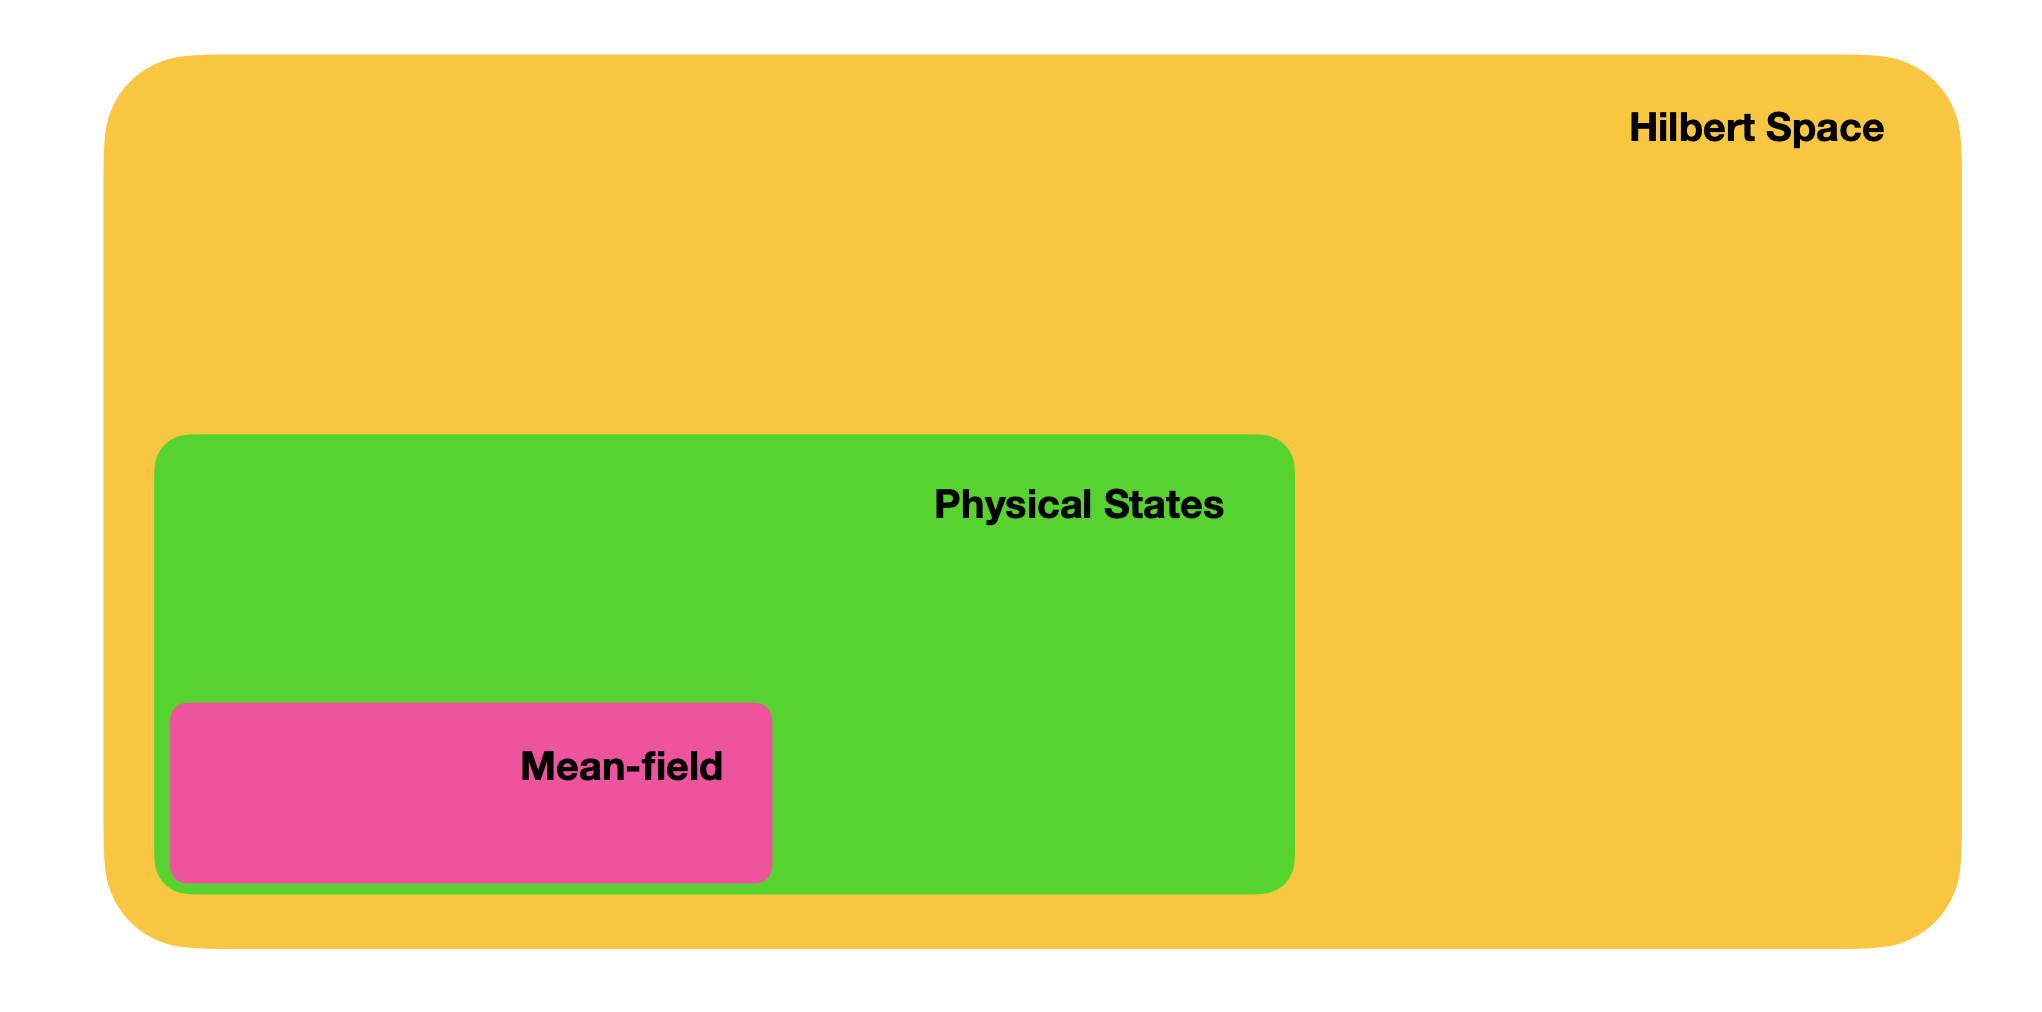
\includegraphics[width=1.0\linewidth]{figures/spaces.png}}

\vspace{6mm}
\end{frame}


\begin{frame}[plain,fragile]
\frametitle{Generative and discriminative models}

%\begin{block}{}
\begin{enumerate}
\item Balance between tractability and flexibility

\item We want to extract information about correlations, to make predictions, quantify uncertainties and express causality

\item How do we represent reliably our effective degrees of freedom?
\end{enumerate}

\noindent
%\end{block}
\end{frame}

\begin{frame}[plain,fragile]
\frametitle{Example of generative modeling, \href{{https://www.oreilly.com/library/view/generative-deep-learning/9781098134174/ch01.html}}{taken from Generative Deep Learning by David Foster}}

\vspace{6mm}

% inline figure
\centerline{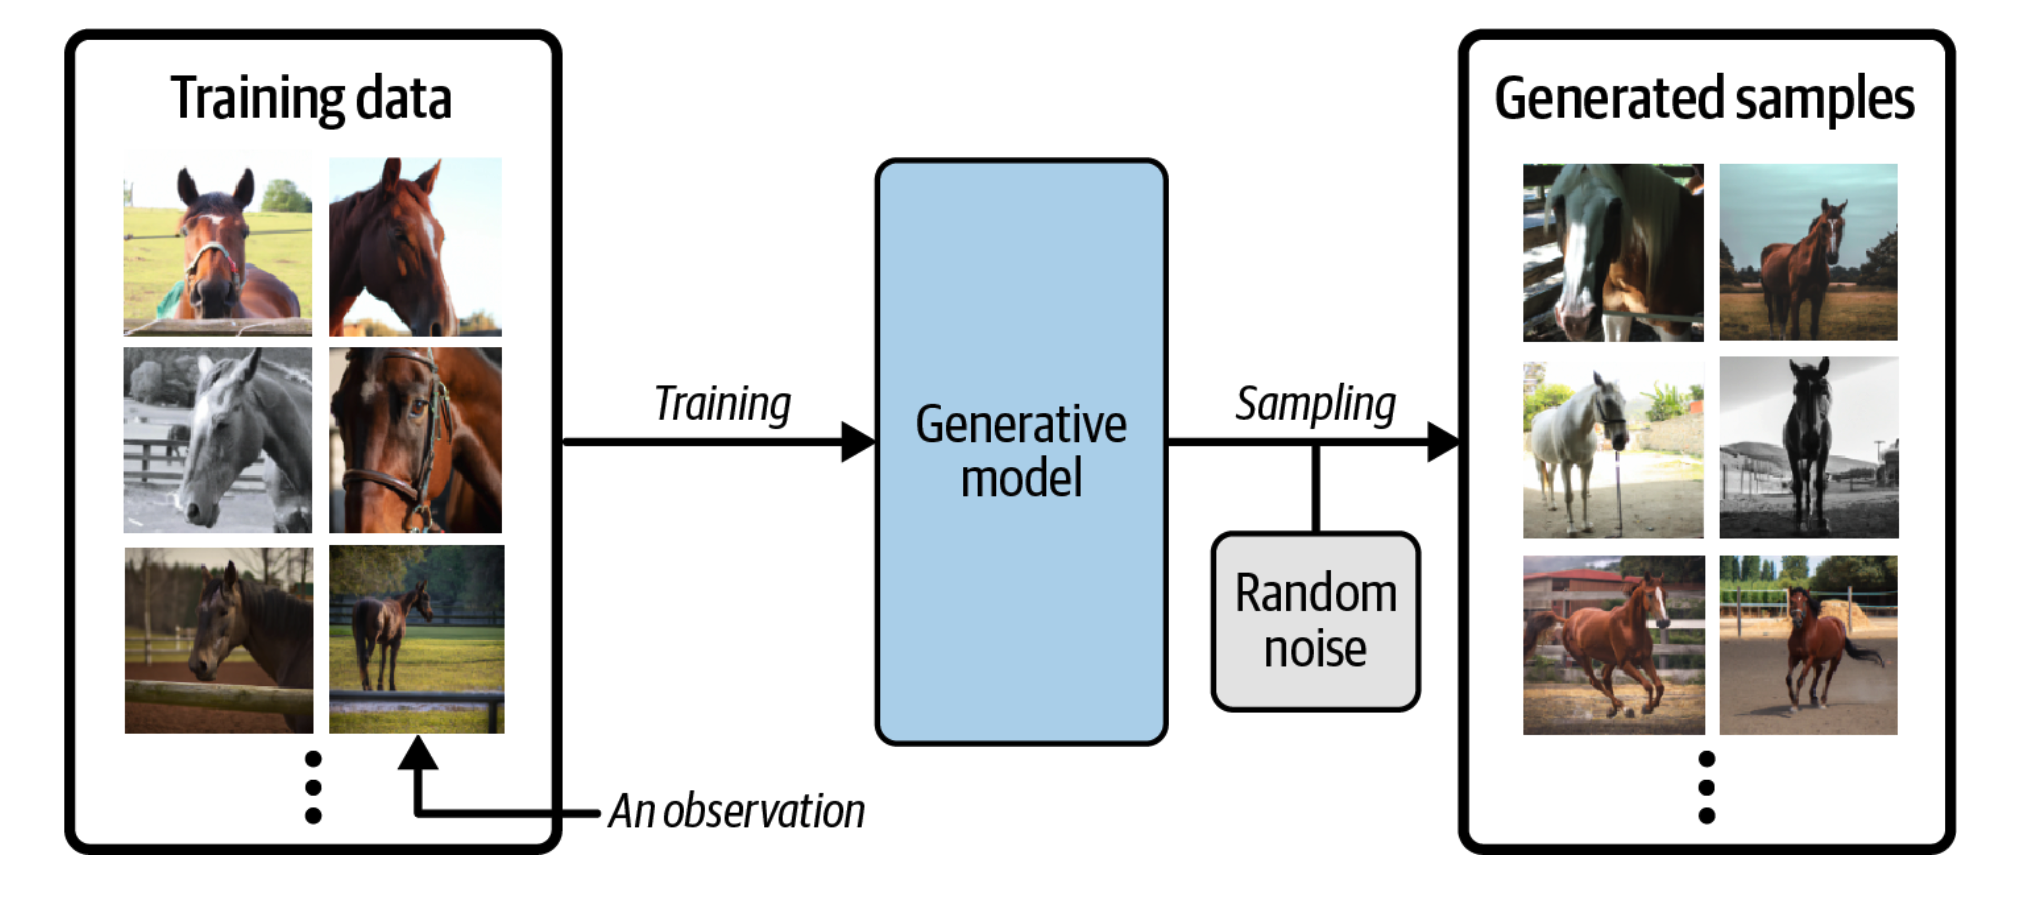
\includegraphics[width=1.0\linewidth]{figures/generativelearning.png}}

\vspace{6mm}
\end{frame}

\begin{frame}[plain,fragile]
\frametitle{Example of discriminative modeling, \href{{https://www.oreilly.com/library/view/generative-deep-learning/9781098134174/ch01.html}}{taken from Generative Deep Learning by David Foster}}

\vspace{6mm}

% inline figure
\centerline{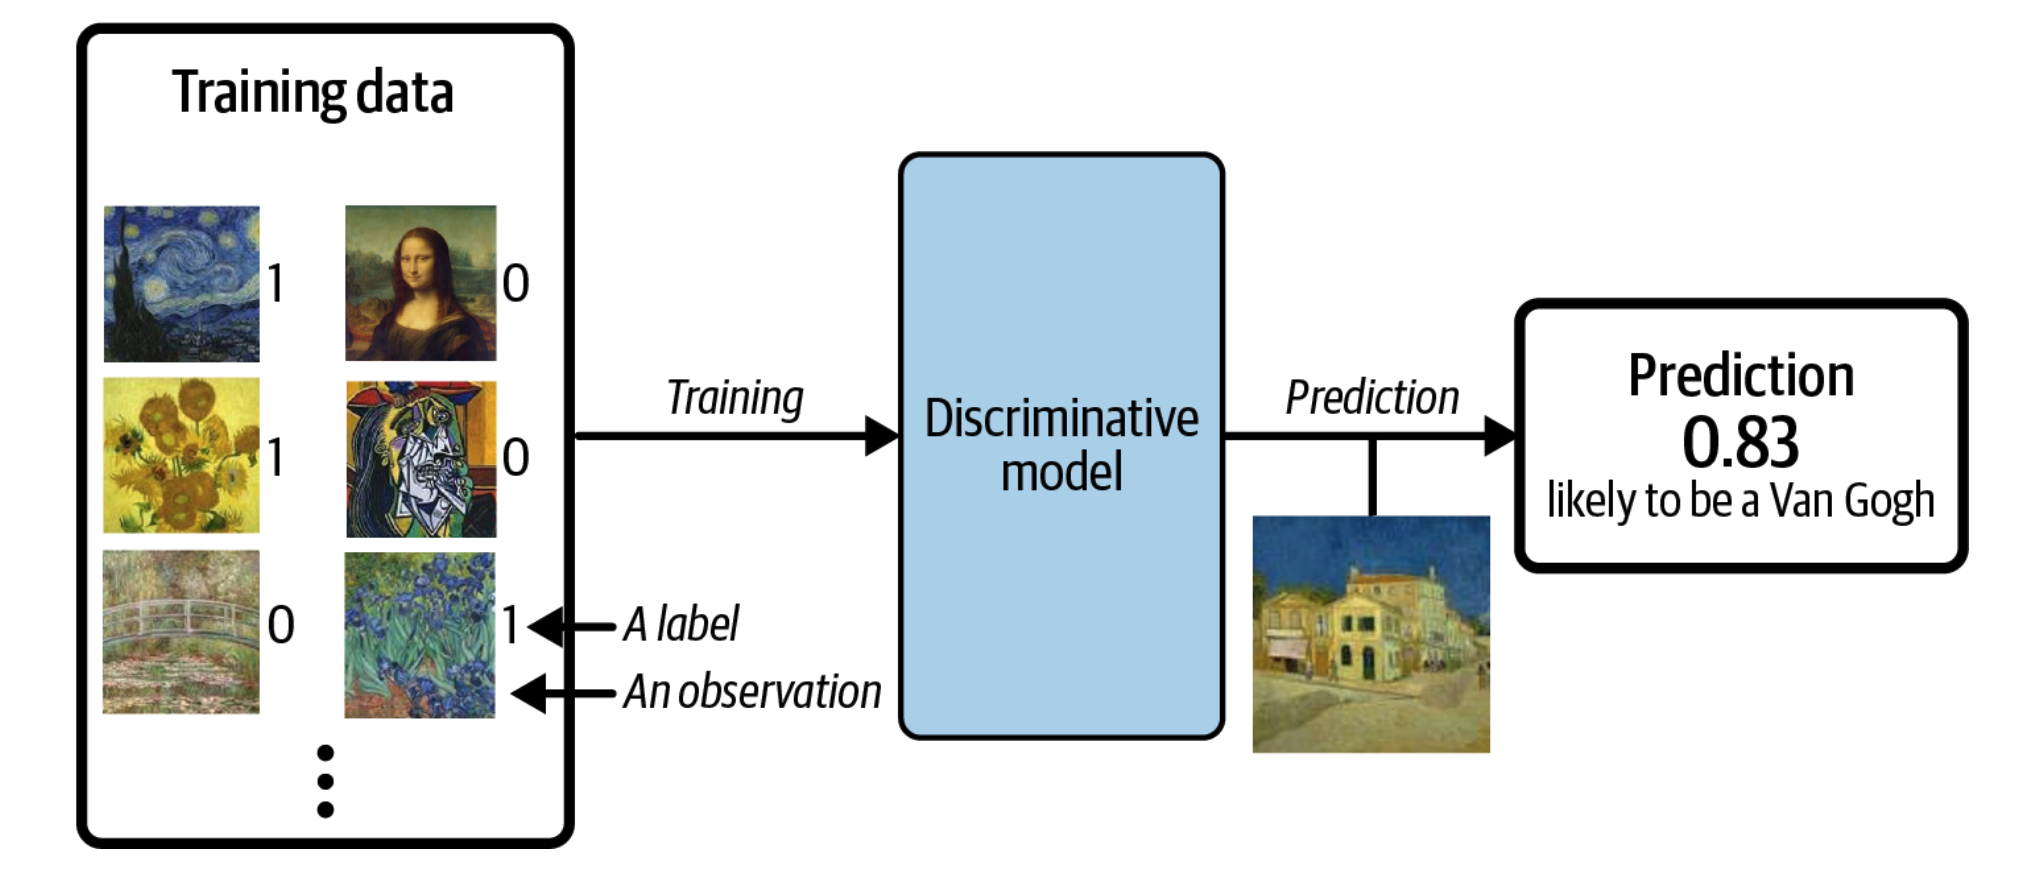
\includegraphics[width=1.0\linewidth]{figures/standarddeeplearning.png}}

\vspace{6mm}
\end{frame}

\begin{frame}[plain,fragile]
\frametitle{Machine learning. A simple perspective on the interface between ML and Physics}

\vspace{6mm}

% inline figure
\centerline{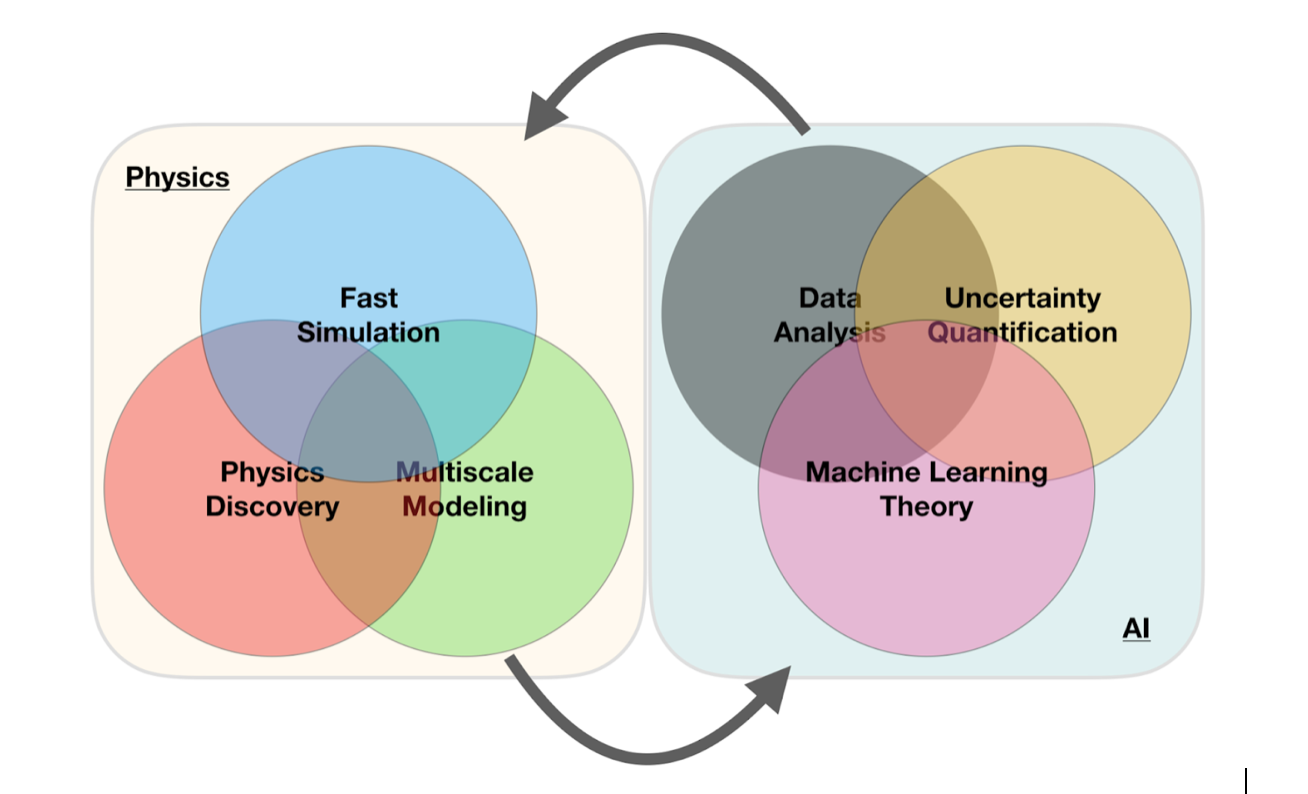
\includegraphics[width=1.0\linewidth]{figures/mlimage.png}}

\vspace{6mm}
\end{frame}







\begin{frame}[plain,fragile]
\frametitle{Many-body physics, Quantum Monte Carlo and deep learning}

%\begin{block}{}
Given a hamiltonian $H$ and a trial wave function $\Psi_T$, the variational principle states that the expectation value of $\langle H \rangle$, defined through 
\[
   \langle E \rangle =
   \frac{\int d\mathbf{R}\Psi^{\ast}_T(\mathbf{R})H(\mathbf{R})\Psi_T(\mathbf{R})}
        {\int d\mathbf{R}\Psi^{\ast}_T(\mathbf{R})\Psi_T(\mathbf{R})},
\]
is an upper bound to the ground state energy $E_0$ of the hamiltonian $H$, that is 
\[
    E_0 \le \langle E \rangle.
\]
In general, the integrals involved in the calculation of various  expectation values  are multi-dimensional ones. Traditional integration methods such as the Gauss-Legendre will not be adequate for say the  computation of the energy of a many-body system.  \textbf{Basic philosophy: Let a neural network find the optimal wave function}
%\end{block}
\end{frame}

\begin{frame}[plain,fragile]
\frametitle{Quantum Monte Carlo Motivation}

%\begin{block}{Basic steps }
Choose a trial wave function
$\psi_T(\mathbf{R})$.
\[
   P(\mathbf{R},\mathbf{\alpha})= \frac{\left|\psi_T(\mathbf{R},\mathbf{\alpha})\right|^2}{\int \left|\psi_T(\mathbf{R},\mathbf{\alpha})\right|^2d\mathbf{R}}.
\]
This is our model, or likelihood/probability distribution function  (PDF). It depends on some variational parameters $\mathbf{\alpha}$.
The approximation to the expectation value of the Hamiltonian is now 
\[
   \langle E[\mathbf{\alpha}] \rangle = 
   \frac{\int d\mathbf{R}\Psi^{\ast}_T(\mathbf{R},\mathbf{\alpha})H(\mathbf{R})\Psi_T(\mathbf{R},\mathbf{\alpha})}
        {\int d\mathbf{R}\Psi^{\ast}_T(\mathbf{R},\mathbf{\alpha})\Psi_T(\mathbf{R},\mathbf{\alpha})}.
\]
%\end{block}
\end{frame}

\begin{frame}[plain,fragile]
\frametitle{Quantum Monte Carlo Motivation}

%\begin{block}{Define a new quantity }
\[
   E_L(\mathbf{R},\mathbf{\alpha})=\frac{1}{\psi_T(\mathbf{R},\mathbf{\alpha})}H\psi_T(\mathbf{R},\mathbf{\alpha}),
\]
called the local energy, which, together with our trial PDF yields
\[
  \langle E[\mathbf{\alpha}] \rangle=\int P(\mathbf{R})E_L(\mathbf{R},\mathbf{\alpha}) d\mathbf{R}\approx \frac{1}{N}\sum_{i=1}^NE_L(\mathbf{R_i},\mathbf{\alpha})
\]
with $N$ being the number of Monte Carlo samples.
%\end{block}
\end{frame}

\begin{frame}[plain,fragile]
\frametitle{Energy derivatives}

%\begin{block}{}
The local energy as function of the variational parameters defines now our \textbf{objective/cost} function.

To find the derivatives of the local energy expectation value as function of the variational parameters, we can use the chain rule and the hermiticity of the Hamiltonian.  

Let us define (with the notation $\langle E[\mathbf{\alpha}]\rangle =\langle  E_L\rangle$)
\[
\bar{E}_{\alpha_i}=\frac{d\langle  E_L\rangle}{d\alpha_i},
\]
as the derivative of the energy with respect to the variational parameter $\alpha_i$
We define also the derivative of the trial function (skipping the subindex $T$) as 
\[
\bar{\Psi}_{i}=\frac{d\Psi}{d\alpha_i}.
\]
%\end{block}
\end{frame}

\begin{frame}[plain,fragile]
\frametitle{Derivatives of the local energy}

%\begin{block}{}
The elements of the gradient of the local energy are 
\[
\bar{E}_{i}= 2\left( \langle \frac{\bar{\Psi}_{i}}{\Psi}E_L\rangle -\langle \frac{\bar{\Psi}_{i}}{\Psi}\rangle\langle E_L \rangle\right).
\]
From a computational point of view it means that you need to compute the expectation values of 
\[
\langle \frac{\bar{\Psi}_{i}}{\Psi}E_L\rangle,
\]
and
\[
\langle \frac{\bar{\Psi}_{i}}{\Psi}\rangle\langle E_L\rangle
\]
These integrals are evaluted using MC intergration (with all its possible error sources). Use methods like stochastic gradient or other minimization methods to find the optimal parameters.
%\end{block}
\end{frame}

\begin{frame}[plain,fragile]
\frametitle{Why Feed Forward Neural Networks (FFNN)?}

According to the \emph{Universal approximation theorem}, a feed-forward
neural network with just a single hidden layer containing a finite
number of neurons can approximate a continuous multidimensional
function to arbitrary accuracy, assuming the activation function for
the hidden layer is a \textbf{non-constant, bounded and
monotonically-increasing continuous function}.
\end{frame}


\begin{frame}[plain,fragile]
\frametitle{Article on wave functions for neural networks}

Fermionic wave functions from neural-network constrained hidden states, 
Javier Robledo Moreno, Giuseppe Carleo, Antoine Georges, and James Stokes,
PNAS {\bf 119} (32) e2122059119 \url{https://doi.org/10.1073/pnas.2122059119}
\end{frame}


\begin{frame}[plain,fragile]
\frametitle{Monte Carlo methods and Neural Networks}

\href{{https://www.sciencedirect.com/science/article/pii/S0370269320305463?via%3Dihub}}{Machine Learning and the Deuteron by Kebble and Rios} and
\href{{https://journals.aps.org/prl/abstract/10.1103/PhysRevLett.127.022502}}{Variational Monte Carlo calculations of $A\le 4$ nuclei with an artificial neural-network correlator ansatz by Adams et al.}

\textbf{Adams et al}:

\begin{align}
H_{LO} &=-\sum_i \frac{{\vec{\nabla}_i^2}}{2m_N}
+\sum_{i<j} {\left(C_1  + C_2\, \vec{\sigma_i}\cdot\vec{\sigma_j}\right)
e^{-r_{ij}^2\Lambda^2 / 4 }}
\nonumber\\
&+D_0 \sum_{i<j<k} \sum_{\text{cyc}}
{e^{-\left(r_{ik}^2+r_{ij}^2\right)\Lambda^2/4}}\,,
\end{align}

where $m_N$ is the mass of the nucleon, $\vec{\sigma_i}$ is the Pauli
matrix acting on nucleon $i$, and $\sum_{\text{cyc}}$ stands for the
cyclic permutation of $i$, $j$, and $k$. The low-energy constants
$C_1$ and $C_2$ are fit to the deuteron binding energy and to the
neutron-neutron scattering length
\end{frame}

\begin{frame}[plain,fragile]
\frametitle{Deep learning neural networks, \href{{https://journals.aps.org/prl/abstract/10.1103/PhysRevLett.127.022502}}{Variational Monte Carlo calculations of $A\le 4$ nuclei with an artificial neural-network correlator ansatz by Adams et al.}}

An appealing feature of the neural network ansatz is that it is more general than the more conventional product of two-
and three-body spin-independent Jastrow functions
\begin{align}
|\Psi_V^J \rangle = \prod_{i<j<k} \Big( 1-\sum_{\text{cyc}} u(r_{ij}) u(r_{jk})\Big) \prod_{i<j} f(r_{ij}) | \Phi\rangle\,,
\end{align}
which is commonly used for nuclear Hamiltonians that do not contain tensor and spin-orbit terms.
The above function is replaced by a multi-layer Neural Network.
\end{frame}

\begin{frame}[plain,fragile]
\frametitle{\href{{https://journals.aps.org/prresearch/pdf/10.1103/PhysRevResearch.5.033062}}{Dilute neutron star matter from neural-network quantum states by Fore et al, Physical Review Research 5, 033062 (2023)} at density $\rho=0.04$ fm$^{-3}$}

%\begin{block}{}

\vspace{6mm}

% inline figure
\centerline{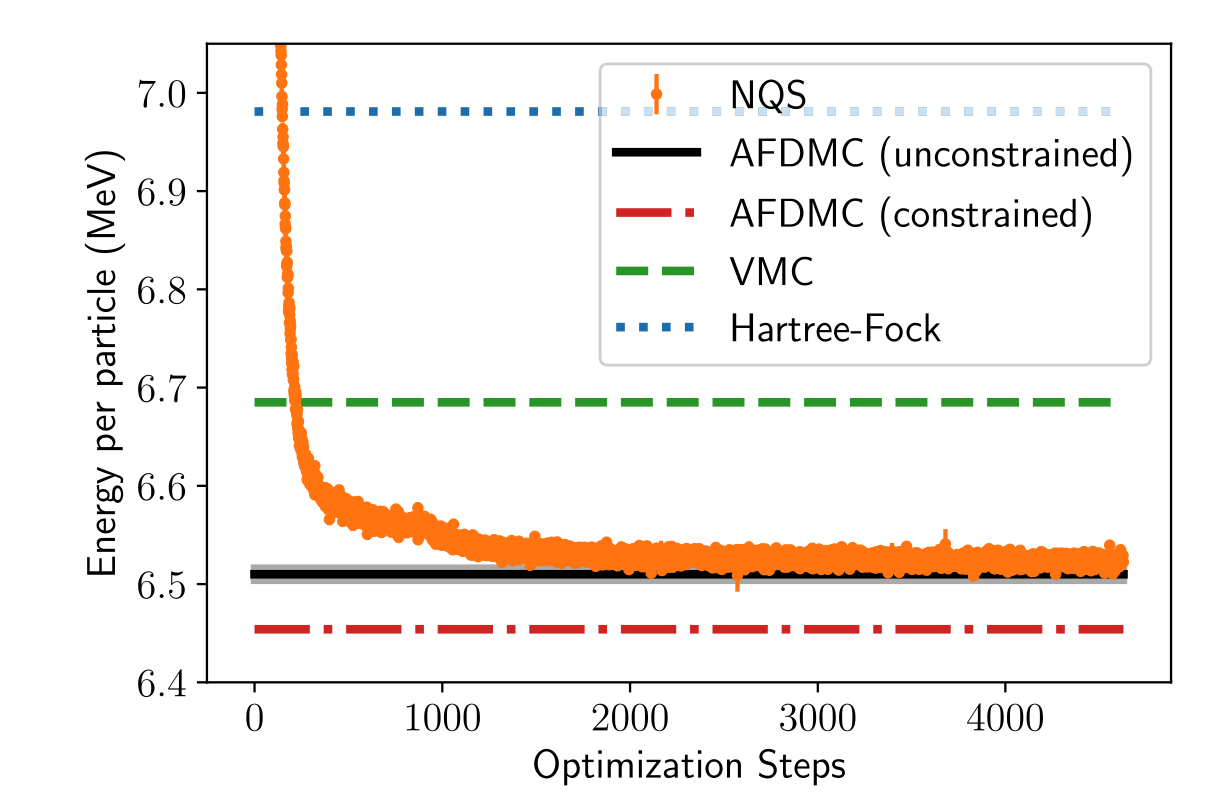
\includegraphics[width=0.8\linewidth]{figures/nmatter.png}}

\vspace{6mm}

%\end{block}
\end{frame}

\begin{frame}[plain,fragile]
\frametitle{Pairing and Spin-singlet and triplet two-body distribution functions at $\rho=0.01$ fm$^{-3}$}

%\begin{block}{}

\vspace{6mm}

% inline figure
\centerline{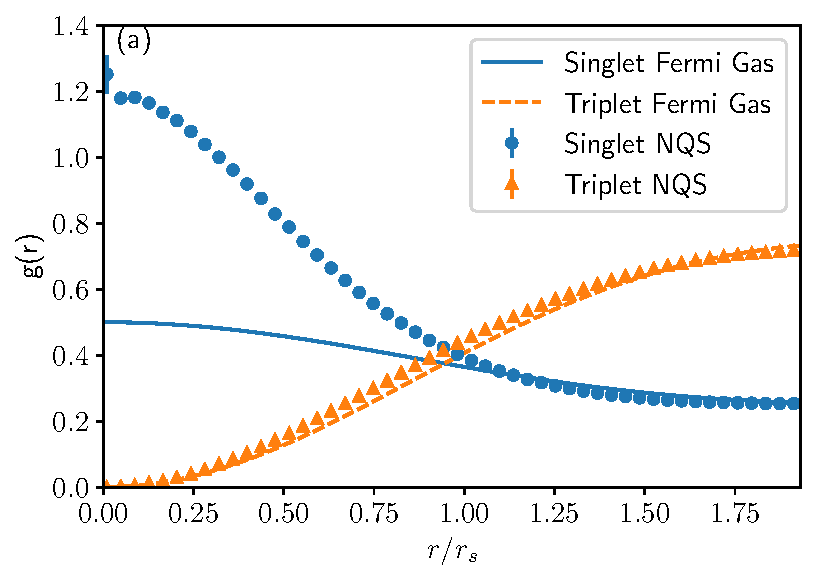
\includegraphics[width=0.8\linewidth]{figures/01_tbd.pdf}}

\vspace{6mm}

%\end{block}
\end{frame}

\begin{frame}[plain,fragile]
\frametitle{Pairing and Spin-singlet and triplet two-body distribution functions at $\rho=0.04$ fm$^{-3}$}

%\begin{block}{}

\vspace{6mm}

% inline figure
\centerline{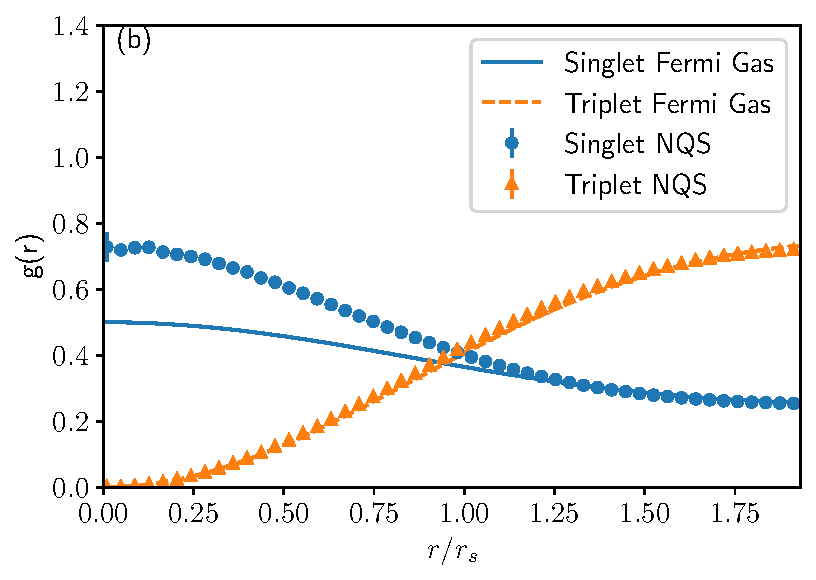
\includegraphics[width=0.8\linewidth]{figures/04_tbd.pdf}}

\vspace{6mm}

%\end{block}
\end{frame}

\begin{frame}[plain,fragile]
\frametitle{Pairing and Spin-singlet and triplet two-body distribution functions at $\rho=0.08$ fm$^{-3}$}

%\begin{block}{}

\vspace{6mm}

% inline figure
\centerline{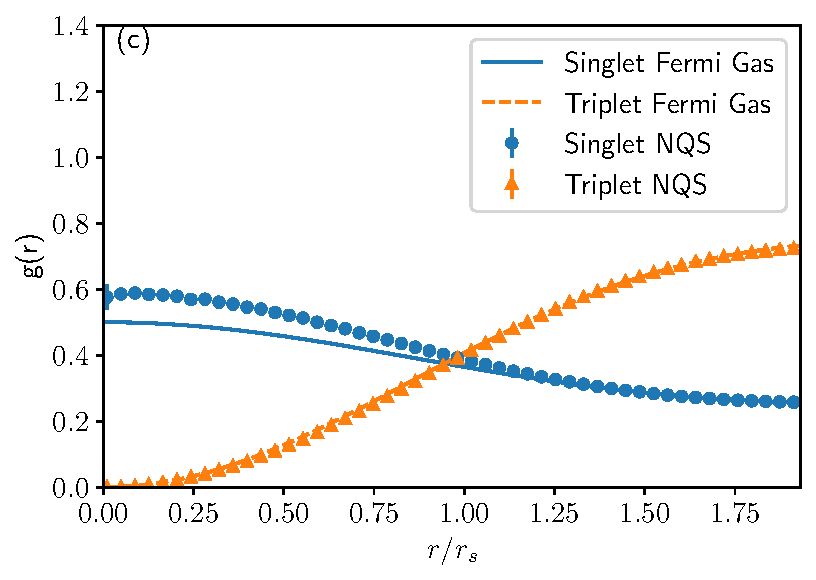
\includegraphics[width=0.8\linewidth]{figures/08_tbd.pdf}}

\vspace{6mm}

%\end{block}
\end{frame}

\begin{frame}[plain,fragile]
\frametitle{The electron gas in three dimensions with $N=14$ electrons (Wigner-Seitz radius $r_s=2$ a.u.), \href{{https://doi.org/10.48550/arXiv.2305.07240}}{Gabriel Pescia, Jane Kim et al.~arXiv.2305.07240,}}

%\begin{block}{}

\vspace{6mm}

% inline figure
\centerline{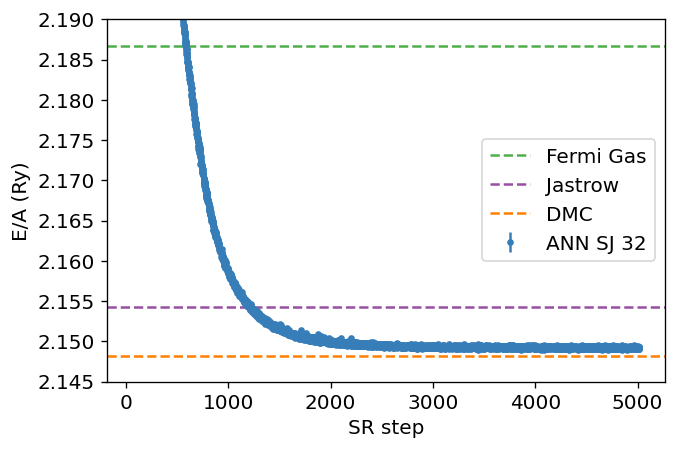
\includegraphics[width=0.8\linewidth]{figures/elgasnew.png}}

\vspace{6mm}

%\end{block}
\end{frame}

\begin{frame}[plain,fragile]
\frametitle{Generical approaches to probability models}

We define a probability
\[
p(x_i,h_j;\mathbf{\Theta}) = \frac{f(x_i,h_j;\mathbf{\Theta})}{Z(\mathbf{\Theta})},
\]
where $f(x_i,h_j;\mathbf{\Theta})$ is a function which we assume is larger or
equal than zero and obeys all properties required for a probability
distribution and $Z(\mathbf{\Theta})$ is a normalization constant. Inspired by
statistical mechanics, we call it often for the partition function.
It is defined as (assuming that we have discrete probability distributions)
\[
Z(\mathbf{\Theta})=\sum_{x_i\in \mathbf{X}}\sum_{h_j\in \mathbf{H}} f(x_i,h_j;\mathbf{\Theta}).
\]
\end{frame}

\begin{frame}[plain,fragile]
\frametitle{Marginal and conditional probabilities}

We can in turn define the marginal probabilities
\[
p(x_i;\mathbf{\Theta}) = \frac{\sum_{h_j\in \mathbf{H}}f(x_i,h_j;\mathbf{\Theta})}{Z(\mathbf{\Theta})},
\]
and 
\[
p(h_i;\mathbf{\Theta}) = \frac{\sum_{x_i\in \mathbf{X}}f(x_i,h_j;\mathbf{\Theta})}{Z(\mathbf{\Theta})}.
\]
\end{frame}

\begin{frame}[plain,fragile]
\frametitle{Change of notation}

A variable like $\mathbf{x}$
represents now a specific \textbf{configuration}. We can generate an infinity
of such configurations. The final partition function is then the sum
over all such possible configurations, that is

\[
Z(\mathbf{\Theta})=\sum_{x_i\in \mathbf{X}}\sum_{h_j\in \mathbf{H}} f(x_i,h_j;\mathbf{\Theta}),
\]
changes to
\[
Z(\mathbf{\Theta})=\sum_{\mathbf{x}}\sum_{\mathbf{h}} f(\mathbf{x},\mathbf{h};\mathbf{\Theta}).
\]
If we have a binary set of variable $x_i$ and $h_j$ and $M$ values of $x_i$ and $N$ values of $h_j$ we have in total $2^M$ and $2^N$ possible $\mathbf{x}$ and $\mathbf{h}$ configurations, respectively.

We see that even for the modest binary case, we can easily approach a
number of configuration which is not possible to deal with.
\end{frame}

\begin{frame}[plain,fragile]
\frametitle{Optimization problem}

At the end, we are not interested in the probabilities of the hidden variables. The probability we thus want to optimize is 
\[
p(\mathbf{X};\mathbf{\Theta})=\prod_{x_i\in \mathbf{X}}p(x_i;\mathbf{\Theta})=\prod_{x_i\in \mathbf{X}}\left(\frac{\sum_{h_j\in \mathbf{H}}f(x_i,h_j;\mathbf{\Theta})}{Z(\mathbf{\Theta})}\right),
\]
which we rewrite as
\[
p(\mathbf{X};\mathbf{\Theta})=\frac{1}{Z(\mathbf{\Theta})}\prod_{x_i\in \mathbf{X}}\left(\sum_{h_j\in \mathbf{H}}f(x_i,h_j;\mathbf{\Theta})\right).
\]
\end{frame}

\begin{frame}[plain,fragile]
\frametitle{Optimizing the logarithm instead}

Computing the derivatives with respect to the parameters $\mathbf{\Theta}$ is
easier (and equivalent) with taking the logarithm of the
probability. We will thus optimize
\[
{\displaystyle \mathrm{arg} \hspace{0.1cm}\max_{\mathbf{\mathbf{\Theta}}\in {\mathbb{R}}^{p}}} \hspace{0.1cm}\log{p(\mathbf{X};\mathbf{\Theta})},
\]
which leads to
\[
\nabla_{\mathbf{\Theta}}\log{p(\mathbf{X};\mathbf{\Theta})}=0.
\]
\end{frame}

\begin{frame}[plain,fragile]
\frametitle{Expression for the gradients}

This leads to the following equation
\[
\nabla_{\mathbf{\Theta}}\log{p(\mathbf{X};\mathbf{\Theta})}=\nabla_{\mathbf{\Theta}}\left(\sum_{x_i\in \mathbf{X}}\log{f(x_i;\mathbf{\Theta})}\right)-\nabla_{\mathbf{\Theta}}\log{Z(\mathbf{\Theta})}=0.
\]

The first term is called the positive phase and we assume that we have a model for the function $f$ from which we can sample values. 
The second term is called the negative phase and is the one which leads to more difficulties.
\end{frame}

\begin{frame}[plain,fragile]
\frametitle{Final expression}

Taking the derivative gives us
\[
\nabla_{\mathbf{\Theta}}\log{Z(\mathbf{\Theta})}=\frac{ \sum_{x_i\in \mathbf{X}}f(x_i;\mathbf{\Theta}) \nabla_{\mathbf{\Theta}}\log{f(x_i;\mathbf{\Theta})}   }{Z(\mathbf{\Theta})}, 
\]
which is the expectation value of $\log{f}$
\[
\nabla_{\mathbf{\Theta}}\log{Z(\mathbf{\Theta})}=\sum_{x_i\sim p}p(x_i;\mathbf{\Theta}) \nabla_{\mathbf{\Theta}}\log{f(x_i;\mathbf{\Theta})},
\]
that is
\[
\nabla_{\mathbf{\Theta}}\log{Z(\mathbf{\Theta})}=\mathbb{E}(\log{f(x_i;\mathbf{\Theta})}).
\]

This quantity is evaluated using Monte Carlo sampling, with Gibbs
sampling as the standard sampling rule.
\end{frame}

\begin{frame}[plain,fragile]
\frametitle{Final expression for the gradients}

This leads to the following equation
\[
\nabla_{\mathbf{\Theta}}\log{p(\mathbf{X};\mathbf{\Theta})}=\nabla_{\mathbf{\Theta}}\left(\sum_{x_i\in \mathbf{X}}\log{f(x_i;\mathbf{\Theta})}\right)-\mathbb{E}_{x\sim p}(\log{f(x_i;\mathbf{\Theta})})=0.
\]
\end{frame}

\begin{frame}[plain,fragile]
\frametitle{Introducing the energy model}

A typical Boltzmann machines employs a probability distribution
\[
p(\mathbf{x},\mathbf{h};\mathbf{\Theta}) = \frac{f(\mathbf{x},\mathbf{h};\mathbf{\Theta})}{Z(\mathbf{\Theta})},
\]
where $f(\mathbf{x},\mathbf{h};\mathbf{\Theta})$ is given by a so-called energy model. If we assume that the random variables $x_i$ and $h_j$ take binary values only, for example $x_i,h_j=\{0,1\}$, we have a so-called binary-binary model where
\[
f(\mathbf{x},\mathbf{h};\mathbf{\Theta})=-E(\mathbf{x}, \mathbf{h};\mathbf{\Theta}) = \sum_{x_i\in \mathbf{X}} x_i a_i+\sum_{h_j\in \mathbf{H}} b_j h_j + \sum_{x_i\in \mathbf{X},h_j\in\mathbf{H}} x_i w_{ij} h_j,
\]
where the set of parameters are given by the biases and weights $\mathbf{\Theta}=\{\mathbf{a},\mathbf{b},\mathbf{W}\}$.
\end{frame}

\begin{frame}[plain,fragile]
\frametitle{More compact notation}

With the above definition we can write the probability as
\[
p(\mathbf{x},\mathbf{h};\mathbf{\Theta}) = \frac{\exp{(\mathbf{a}^T\mathbf{x}+\mathbf{b}^T\mathbf{h}+\mathbf{x}^T\mathbf{W}\mathbf{h})}}{Z(\mathbf{\Theta})},
\]
where the biases $\mathbf{a}$ and $\mathbf{h}$ and the weights defined by the matrix $\mathbf{W}$ are the parameters we need to optimize.
\end{frame}

\begin{frame}[plain,fragile]
\frametitle{Examples of gradient expressions}

Since the binary-binary energy model is linear in the parameters $a_i$, $b_j$ and
$w_{ij}$, it is easy to see that the derivatives with respect to the
various optimization parameters yield expressions used in the
evaluation of gradients like
\[
\frac{\partial E(\mathbf{x}, \mathbf{h};\mathbf{\Theta})}{\partial w_{ij}}=-x_ih_j,
\]
and
\[
\frac{\partial E(\mathbf{x}, \mathbf{h};\mathbf{\Theta})}{\partial a_i}=-x_i,
\]
and
\[
\frac{\partial E(\mathbf{x}, \mathbf{h};\mathbf{\Theta})}{\partial b_j}=-h_j.
\]
\end{frame}

\begin{frame}[plain,fragile]
\frametitle{Network Elements, the energy function}

The function $E(\mathbf{x},\mathbf{h},\mathbf{\Theta})$ gives the \textbf{energy} of a
configuration (pair of vectors) $(\mathbf{x}, \mathbf{h})$. The lower
the energy of a configuration, the higher the probability of it. This
function also depends on the parameters $\mathbf{a}$, $\mathbf{b}$ and
$W$. Thus, when we adjust them during the learning procedure, we are
adjusting the energy function to best fit our problem.
\end{frame}

\begin{frame}[plain,fragile]
\frametitle{Defining different types of RBMs}

There are different variants of RBMs, and the differences lie in the types of visible and hidden units we choose as well as in the implementation of the energy function $E(\mathbf{x},\mathbf{h},\mathbf{\Theta})$. The connection between the nodes in the two layers is given by the weights $w_{ij}$. 

%\begin{block}{Binary-Binary RBM: }

RBMs were first developed using binary units in both the visible and hidden layer. The corresponding energy function is defined as follows:
\begin{align*}
	E(\mathbf{x}, \mathbf{h},\mathbf{\Theta}) = - \sum_i^M x_i a_i- \sum_j^N b_j h_j - \sum_{i,j}^{M,N} x_i w_{ij} h_j,
\end{align*}
where the binary values taken on by the nodes are most commonly 0 and 1.
%\end{block}
\end{frame}

\begin{frame}[plain,fragile]
\frametitle{Gaussian-binary RBM}

Another varient is the RBM where the visible units are Gaussian while the hidden units remain binary:
\begin{align*}
	E(\mathbf{x}, \mathbf{h},\mathbf{\Theta}) = \sum_i^M \frac{(x_i - a_i)^2}{2\sigma_i^2} - \sum_j^N b_j h_j - \sum_{i,j}^{M,N} \frac{x_i w_{ij} h_j}{\sigma_i^2}. 
\end{align*}

This type of RBMs are useful when we model continuous data (i.e., we wish $\mathbf{x}$ to be continuous). The paramater $\sigma_i^2$ is meant to represent a variance and is foten just set to one.
\end{frame}

\begin{frame}[plain,fragile]
\frametitle{\href{{https://doi.org/10.3389/fphy.2023.1061580}}{Efficient solutions of fermionic systems using artificial neural networks, Nordhagen et al, Frontiers in Physics 11, 2023}}

The Hamiltonian of the quantum dot is given by
\[ \hat{H} = \hat{H}_0 + \hat{V}, 
\]
where $\hat{H}_0$ is the many-body HO Hamiltonian, and $\hat{V}$ is the
inter-electron Coulomb interactions. In dimensionless units,
\[ \hat{V}= \sum_{i < j}^N \frac{1}{r_{ij}},
\]
with $r_{ij}=\sqrt{\mathbf{r}_i^2 - \mathbf{r}_j^2}$.

Separable Hamiltonian with the relative motion part ($r_{ij}=r$)
\[ 
\hat{H}_r=-\nabla^2_r + \frac{1}{4}\omega^2r^2+ \frac{1}{r},
\]
Analytical solutions in two and three dimensions (\href{{https://journals.aps.org/pra/abstract/10.1103/PhysRevA.48.3561}}{M. Taut 1993 and 1994}).
\end{frame}

\begin{frame}[plain,fragile]
\frametitle{Quantum dots and Boltzmann machines, onebody densities $N=6$, $\hbar\omega=0.1$ a.u.}

%\begin{block}{}

\vspace{6mm}

% inline figure
\centerline{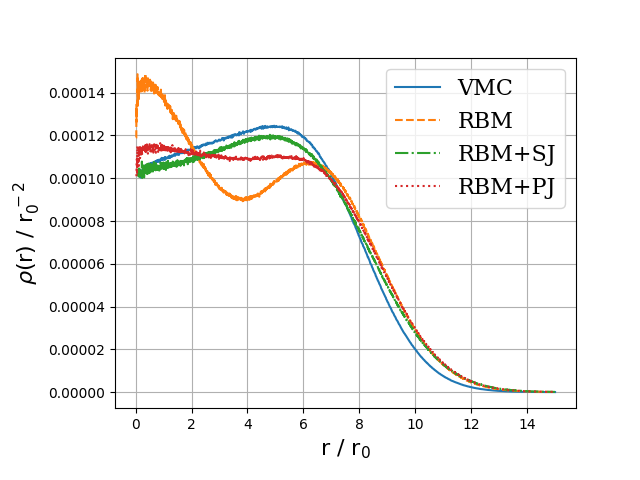
\includegraphics[width=0.9\linewidth]{figures/OB6hw01.png}}

\vspace{6mm}

%\end{block}
\end{frame}

\begin{frame}[plain,fragile]
\frametitle{Onebody densities $N=30$, $\hbar\omega=1.0$ a.u.}

%\begin{block}{}

\vspace{6mm}

% inline figure
\centerline{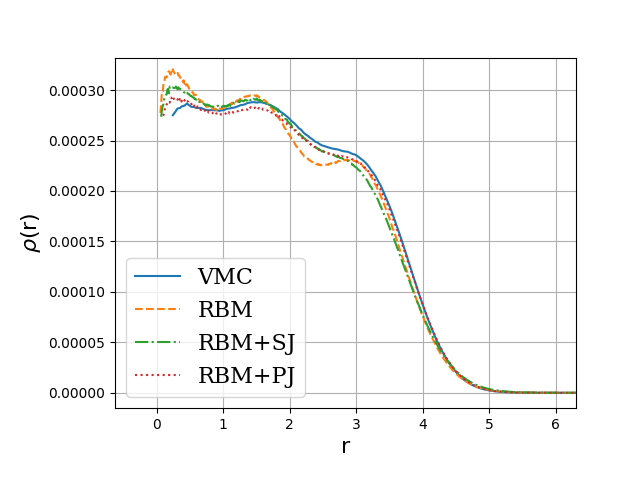
\includegraphics[width=0.9\linewidth]{figures/OB30hw1.png}}

\vspace{6mm}

%\end{block}
\end{frame}

\begin{frame}[plain,fragile]
\frametitle{Expectation values as functions of the oscillator frequency}

%\begin{block}{}

\vspace{6mm}

% inline figure
\centerline{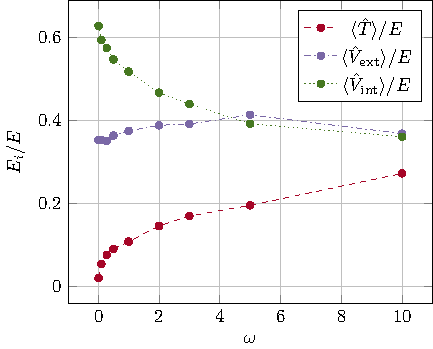
\includegraphics[width=0.8\linewidth]{figures/virialtheorem.pdf}}

\vspace{6mm}

%\end{block}
\end{frame}

\begin{frame}[t]{Parametric Matrix Models, some references}
  \begin{itemize}
    \item Parametric Matrix Models, Patrick Cook, Danny Jammooa, MHJ, Dean Lee and Daniel Lee, \href{{https://arxiv.org/abs/2401.11694}}{\nolinkurl{https://arxiv.org/abs/2401.11694}}. 
    \item Recent application: Emulators for scarce and noisy data, application to auxiliary field diffusion Monte Carlo for the deuteron, Rahul Somasundaram, Cassandra L. Armstrong, Pablo Giuliani, Kyle Godbey, Stefano Gandolfi, Ingo Tews \url{https://arxiv.org/abs/2404.11566}
    \end{itemize}
\end{frame}



\begin{frame}[t]{Parametric Matrix Models}
    \begin{itemize}
        \item Parametric Matrix Models (PMMs) are powerful for sparse and noisy data
        \item This strongly suggests they are parameter- and computationally-efficient and robust
    \end{itemize}
    \begin{shaded*}
        \textbf{Does this advantage generalize to general machine learning problems?}
    \end{shaded*}
\end{frame}

\begin{frame}[t]{Current ``Solution''}
    More parameters, more data, more compute, more time
    \begin{figure}
        \centering
        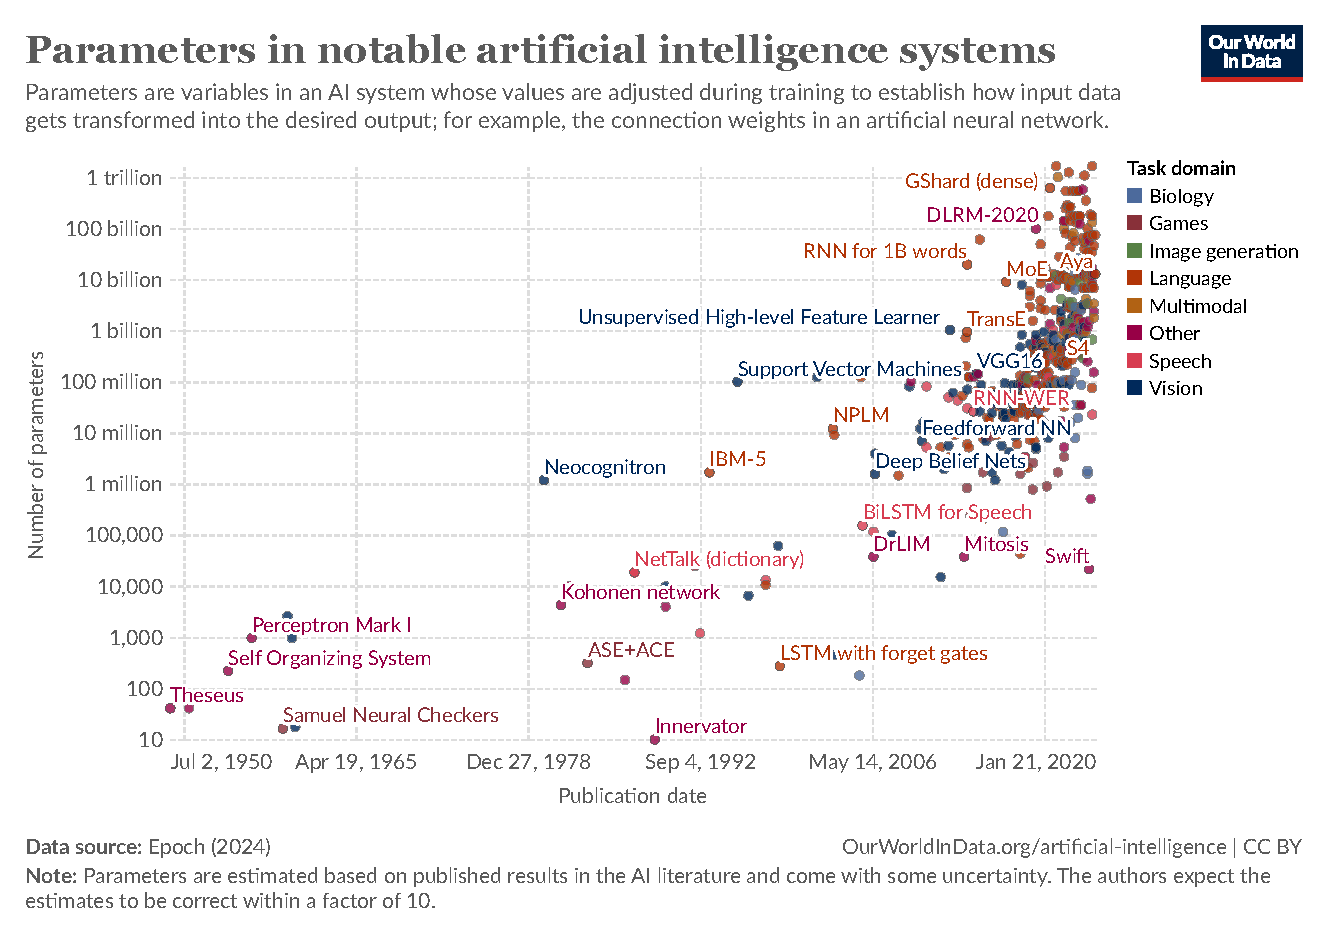
\includegraphics[height=0.7\textheight]{./Figures/artificial-intelligence-parameter-count.pdf}
    \end{figure}
\end{frame}


\begin{frame}[plain,fragile]
\frametitle{Parametric Matrix Models for effective Hamiltonians}

Given data for $k$ energies and $k$ observables in the ground state of a Hamiltonian that is a function of some constants
\[
\begin{aligned}
    H(\mathbf{x}) &= H_0 +\sum_jx_jH_j\\
      \hat{y}(\mathbf{x}) &= [\hat{E}_k(\mathbf{x}),\langle\psi_0(\mathbf{x})|\hat{O}_k|\psi_0(\mathbf{x})\rangle]
      \end{aligned}
\]
\end{frame}

\begin{frame}[plain,fragile]
\frametitle{Model with same structure}

We form a PMM with same structure
\[
    M(\mathbf{x}) = \underline{M_0} + \sum_jx_j\underline{M_j}
\]
and calculate its $k$ energies and $k$ observables
\begin{equation}
    y(\mathbf{x}) = [E_k(\mathbf{c}),\langle\phi_0(\mathbf{c})|\underline{O}_k|\phi_0(\mathbf{c})\rangle]
\end{equation}
where $\underline{M_0},\underline{M}_j,\underline{O}\in\mathbf{C}^{\overline{n}\times\overline{n}}$ are Hermitian matrices.
\end{frame}


\begin{frame}[plain,fragile]
\frametitle{Simple labeling}

The trainable parameters are trained by minimizing the mean squared
error over all $N$ training points.

\[
    \begin{aligned}
        \mathcal{L} = \frac{1}{N}\sum^N_i(\hat{y}_k(\mathbf{x}_i)-y_k(\mathbf{x}_i))^2,
    \end{aligned}
\]
where $\hat{y}_k(\mathbf{x})$ is the true data, and $y_k(\mathbf{x})$ corresponds to the output of the PMM.
\end{frame}



\section{From Physics}
\subsection{to Whatever}
\begin{frame}[t]{Generalizing PMMs}
    \vspace{-3em}
    \begin{columns}[t]
        \begin{column}{0.5\textwidth}
            \begin{shaded*}
                \centering
                \textbf{Make a ``Hamiltonian''}
            \end{shaded*}
            \vspace{-1em}
            \visible<3->{%
                \begin{equation*}
                    H(\mathbf{x})
                \end{equation*}
            }
            \vspace{-1em}

            \visible<5->{%
                \noindent\rule{\textwidth}{0.4pt}
                \begin{equation*}
                    H(\mathbf{x}) = \trainable{H_0} + \sum_i x_i \trainable{H_i}
                \end{equation*}
            }
            \visible<6->{%
                \begin{equation*}
                    H(\mathbf{x}) = \trainable{H_0} + \mathbf{x}\trainable{H_1}\mathbf{x}^\dagger
                \end{equation*}
            }
            \visible<7->{%
                \begin{equation*}
                    H(\mathbf{X}) = \trainable{H_0} + \trainable{H_1} \mathbf{X} \trainable{H_1}^\dagger
                \end{equation*}
            }
        \end{column}
        \begin{column}{0.5\textwidth}
            \begin{shaded*}
                \centering
                \textbf{Use its eigensystem}
            \end{shaded*}
            \vspace{-1em}
            \visible<4->{%
                \begin{equation*}
                    H(\mathbf{x}) \rightarrow V\Lambda V^\dagger \rightarrow \mathbf{z}
                \end{equation*}
            }
            \vspace{-1em}

            \visible<8->{%
                \noindent\rule{\textwidth}{0.4pt}
                \begin{equation*}
                    \mathbf{z} = \mathrm{diag}\left(\Lambda\right)
                \end{equation*}
            }
            \visible<9->{%
                \begin{equation*}
                    z_i = v_i^\dagger \trainable{\Delta} v_i
                \end{equation*}
            }
            \visible<10->{%
                \begin{equation*}
                    z_i = v_0^\dagger \trainable{\Delta_i} v_0
                \end{equation*}
            }

        \end{column}
    \end{columns}

\end{frame}





\subsection{Results}
\begin{frame}[t]{2D Surfaces}
    \pause
    \only<2>{%
        Franke's Bivariate Test Function
        \begin{figure}
            \centering
            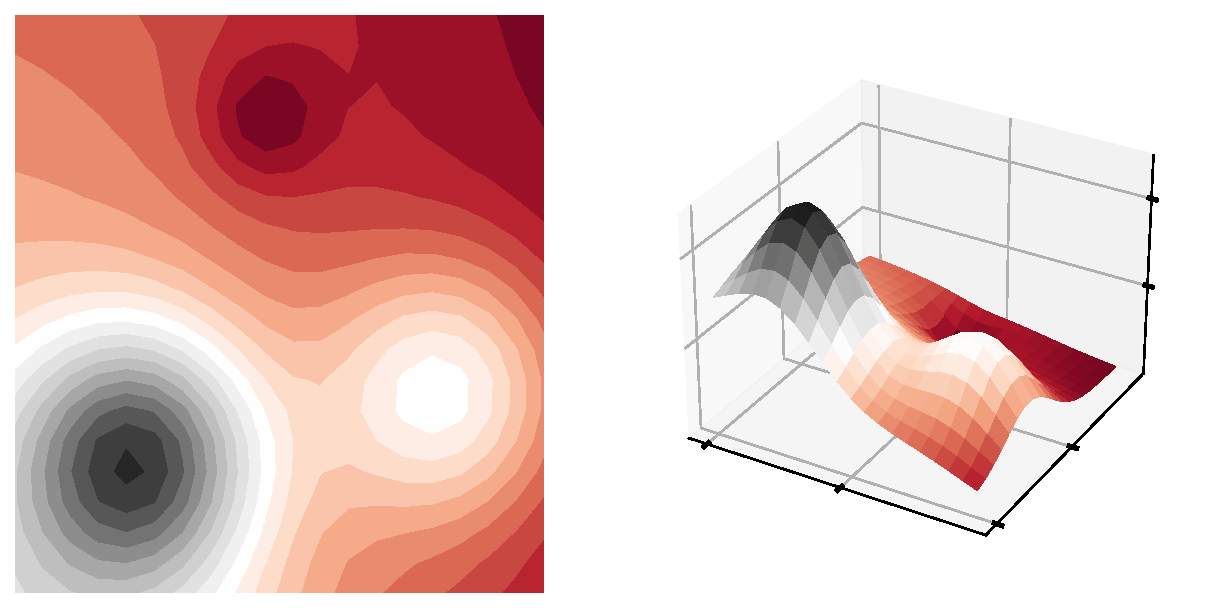
\includegraphics[width=0.8\textwidth]{./Figures/franke.pdf}
        \end{figure}
    }
    \only<3>{%
        Franke's Bivariate Test Function
        \begin{figure}
            \centering
            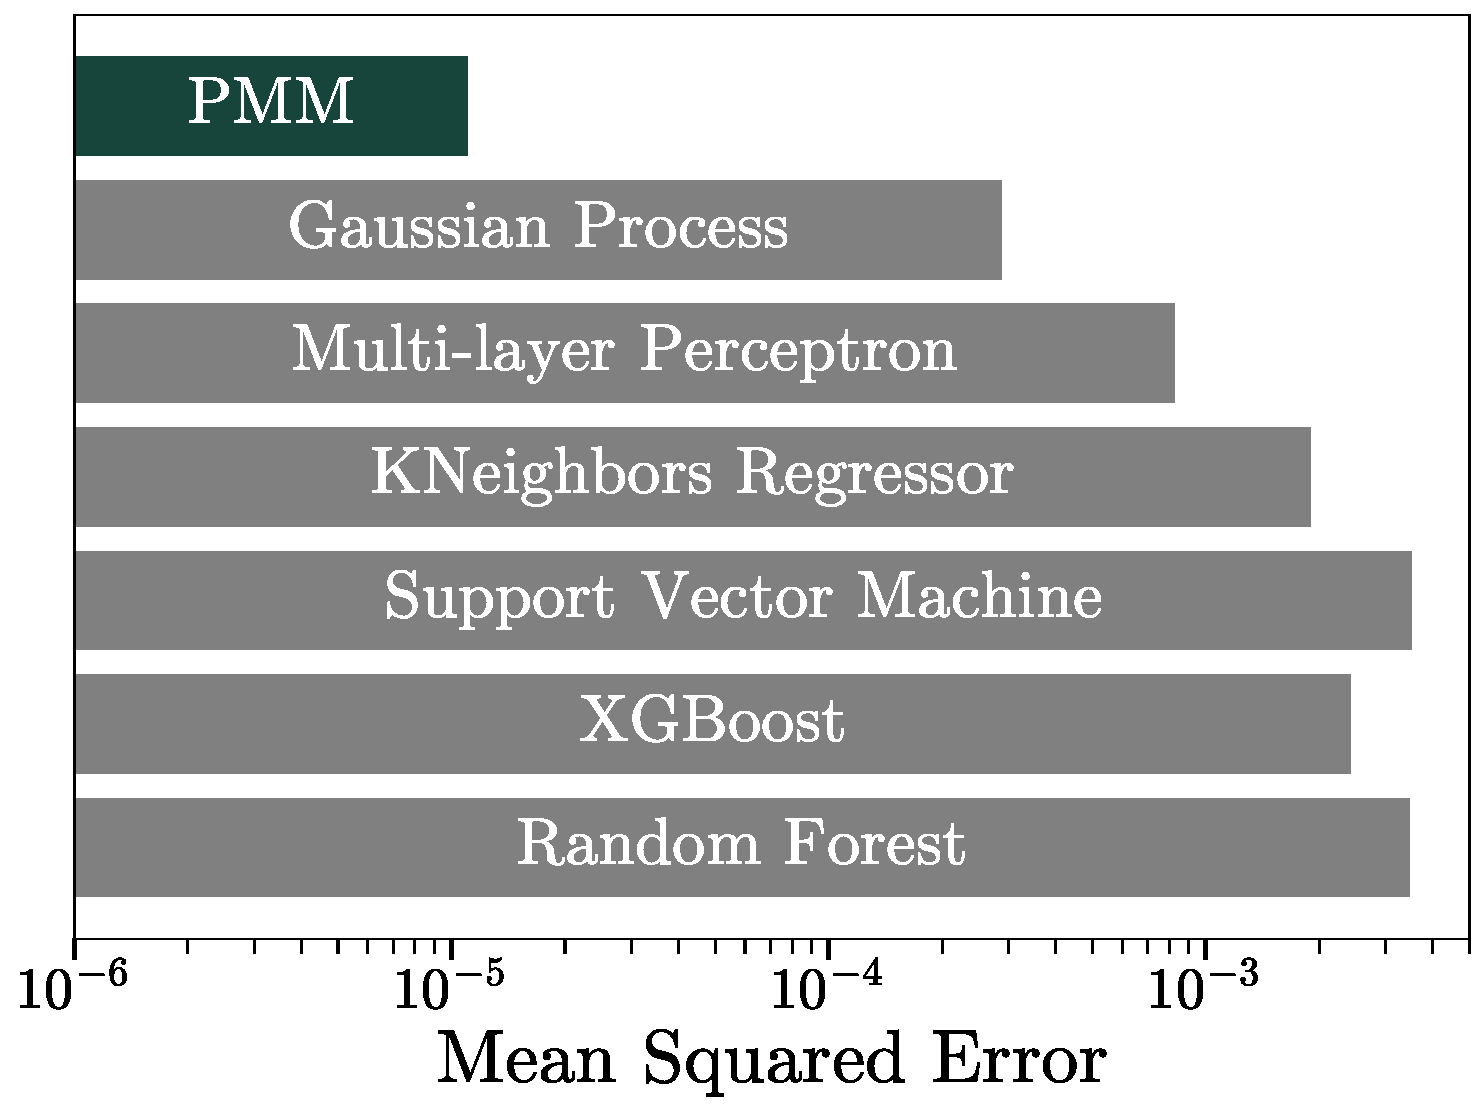
\includegraphics[width=0.7\textwidth]{./Figures/MSE_Franke_function.pdf}
        \end{figure}
    }
    \only<4>{%
        Cliff Function
        \begin{figure}
            \centering
            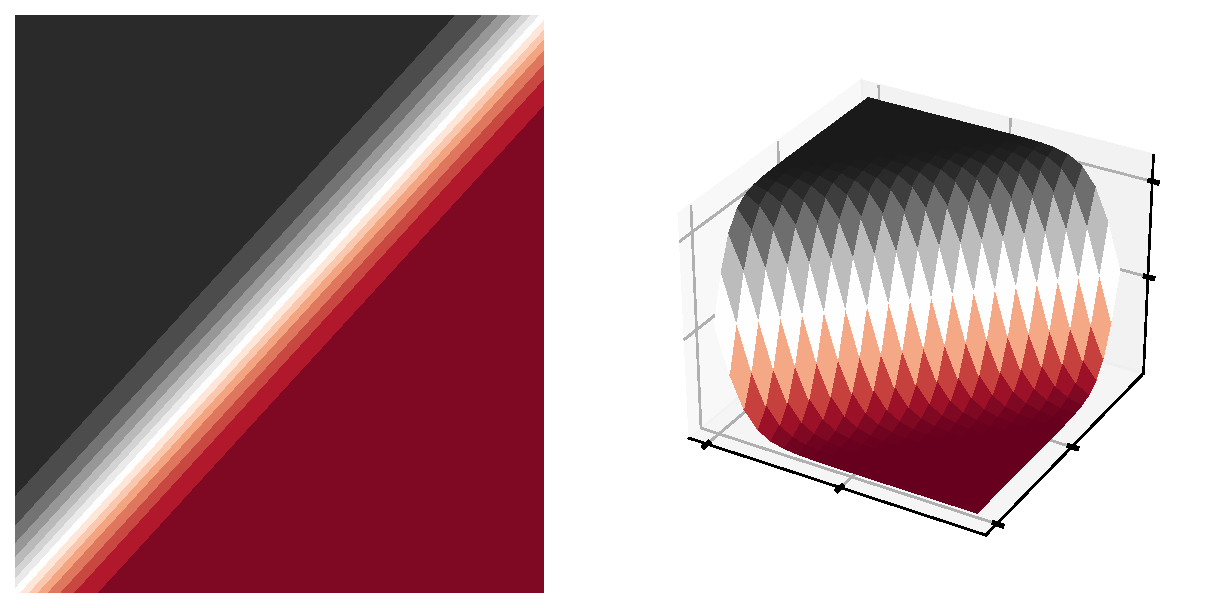
\includegraphics[width=0.8\textwidth]{./Figures/cliff.pdf}
        \end{figure}
    }
    \only<5>{%
        Cliff Function
        \begin{figure}
            \centering
            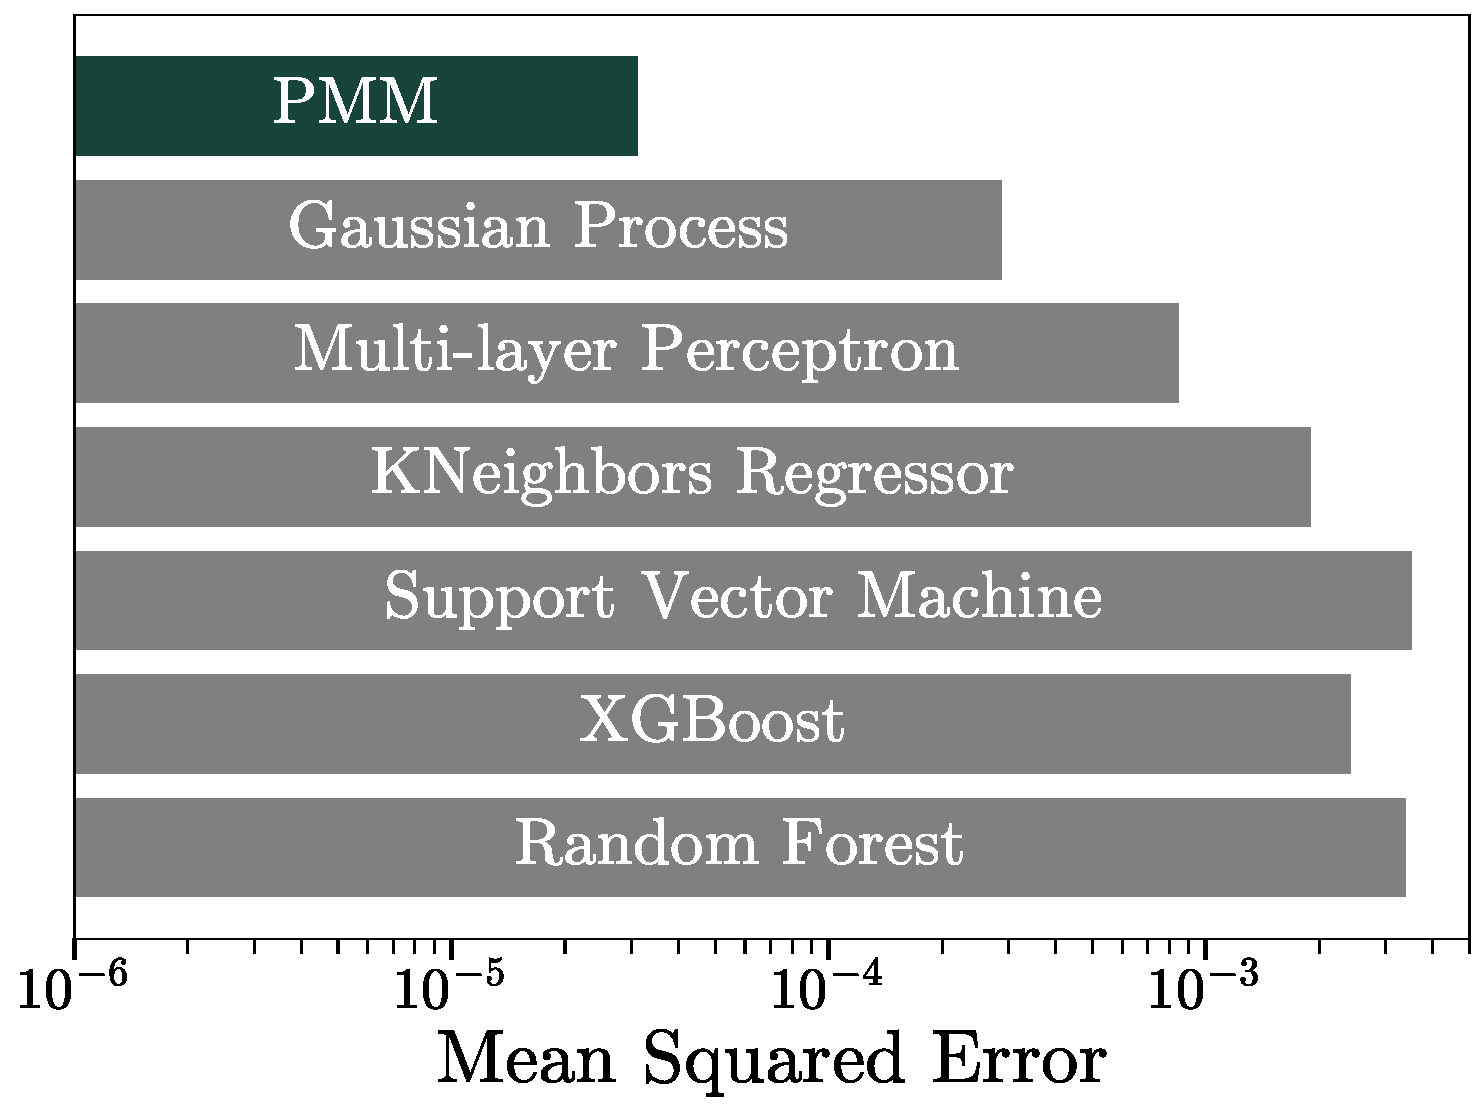
\includegraphics[width=0.7\textwidth]{./Figures/MSE_Cliff.pdf}
        \end{figure}
    }
    \only<6>{%
        Runge Function
        \begin{figure}
            \centering
            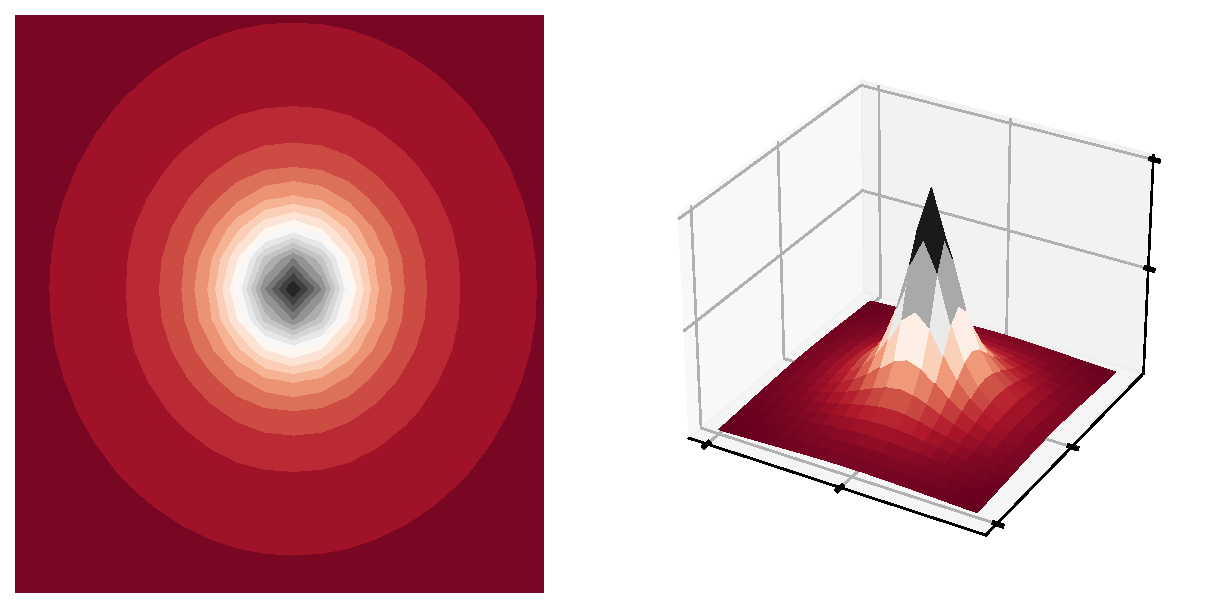
\includegraphics[width=0.8\textwidth]{./Figures/runge.pdf}
        \end{figure}
    }
    \only<7>{%
        Runge Function
        \begin{figure}
            \centering
            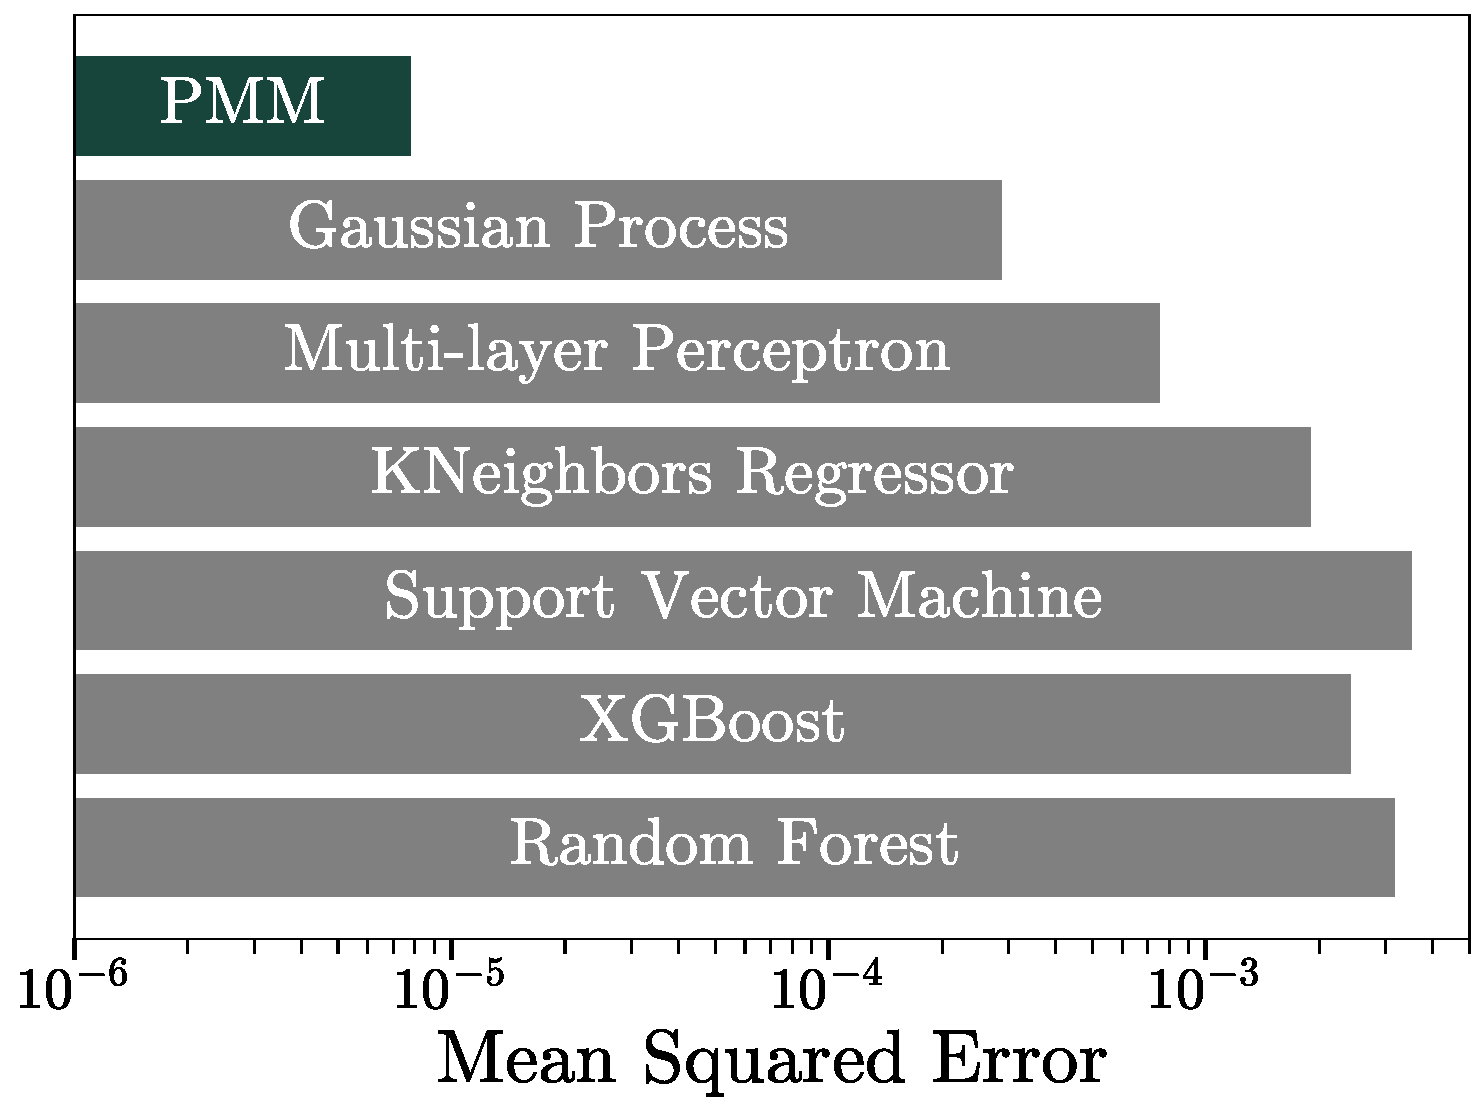
\includegraphics[width=0.7\textwidth]{./Figures/MSE_Runge_function.pdf}
        \end{figure}
    }

\end{frame}




\begin{frame}[plain,fragile]
\frametitle{Observations (or conclusions if you prefer)}

\begin{block}{}
\begin{itemize}
\item Need for AI/Machine Learning in physics, lots of ongoing activities

\item To solve many complex problems and facilitate discoveries, multidisciplinary efforts are required involving scientists in  physics, statistics, computational science, applied math and other fields.

\item There is a need for  focused AI/ML learning efforts that will benefit accelerator science and experimental and theoretical programs
\end{itemize}

\noindent
\end{block}
\end{frame}



\begin{frame}[plain,fragile]
\frametitle{More observations}

\begin{block}{}
\begin{itemize}
\item How do we develop insights, competences, knowledge in ML/AI  that can advance a given field?
\begin{itemize}

  \item For example: Can we use ML to find out which correlations are relevant and thereby diminish the dimensionality problem in standard many-body  theories?

  \item Can we use AI/ML in detector analysis, accelerator design, analysis of experimental data and more?

  \item Can we use AL/ML to carry out reliable extrapolations by using current experimental knowledge and current theoretical models?

\end{itemize}

\noindent
\item The community needs to invest in relevant educational efforts and training of scientists with knowledge in AI/ML. These are great challenges to the CS and DS communities

\item Quantum computing and quantum machine learning not discussed here

\item Most likely tons of things I have forgotten
\end{itemize}

\noindent
\end{block}
\end{frame}
\begin{frame}[plain,fragile]
\frametitle{Possible start to raise awareness about ML in our own field}

\begin{block}{}
\begin{itemize}
\item Make an ML challenge in your own field a la \href{{https://home.cern/news/news/computing/higgs-boson-machine-learning-challenge}}{Learn\
ing to discover: the Higgs boson machine learning challenge}. Alternatively go to kaggle.com at \href{{https://www.kaggle.com/c/higgs-boson}}\
{\nolinkurl{https://www.kaggle.com/c/higgs-boson}}

\item HEP@CERN and HEP in general have made significant impacts in the field of machine learning and AI. Something to learn from
\end{itemize}

\noindent
\end{block}
\end{frame}


\end{document}


